\documentclass[11pt, dvipdfmx]{jarticle}

\usepackage[dvipdfmx]{graphicx}
\newcommand{\setPicture}[1]{\includegraphics[width=1\linewidth]{chapters/picture/#1}}
\usepackage{sty/fancyheadings}
\usepackage{sty/sotsuron2009}
\usepackage{here}
\usepackage{ascmac}
\usepackage[subrefformat=parens]{subcaption}
\usepackage{here}
\usepackage{cite}
\usepackage{amsmath}
\usepackage{pdfpages}
\pagestyle{empty}
\usepackage{bm}
\usepackage{comment}
\usepackage{url}
\linesparpage{40}
%\makeatletter
%\renewcommand{\theequation}{
%\thesection.\arabic{equation}}
%\@addtoreset{equation}{section}
%\makeatother
\pagestyle{fancy}

\newcommand{\argmin}{\mathop{\rm arg~min}\limits}
\setcounter{topnumber}{5}
\setcounter{bottomnumber}{5}
\setcounter{totalnumber}{10}
\renewcommand{\textfraction}{0.0}
\renewcommand{\topfraction}{1.0}

\newcommand{\Section}[1]{\section*{#1}
\addcontentsline{toc}{section}{#1}}
\newcommand{\Subsection}[1]{\section*{#1}
\addcontentsline{toc}{subsection}{#1}}
\renewcommand{\refname}{}


\begin{document}

\begin{comment}
\title{
 \LARGE
 % 卒論和文タイトル
 \\ \\
 \large
 % 卒論英文タイトル
}

\author{
 研究者 高専 太郎\\
 指導教員 中西 大輔\\ \\
 松江工業高等専門学校\\
 電子制御工学科\\ \\
}

\date{平成29年2月13日}

\maketitle
\end{comment}

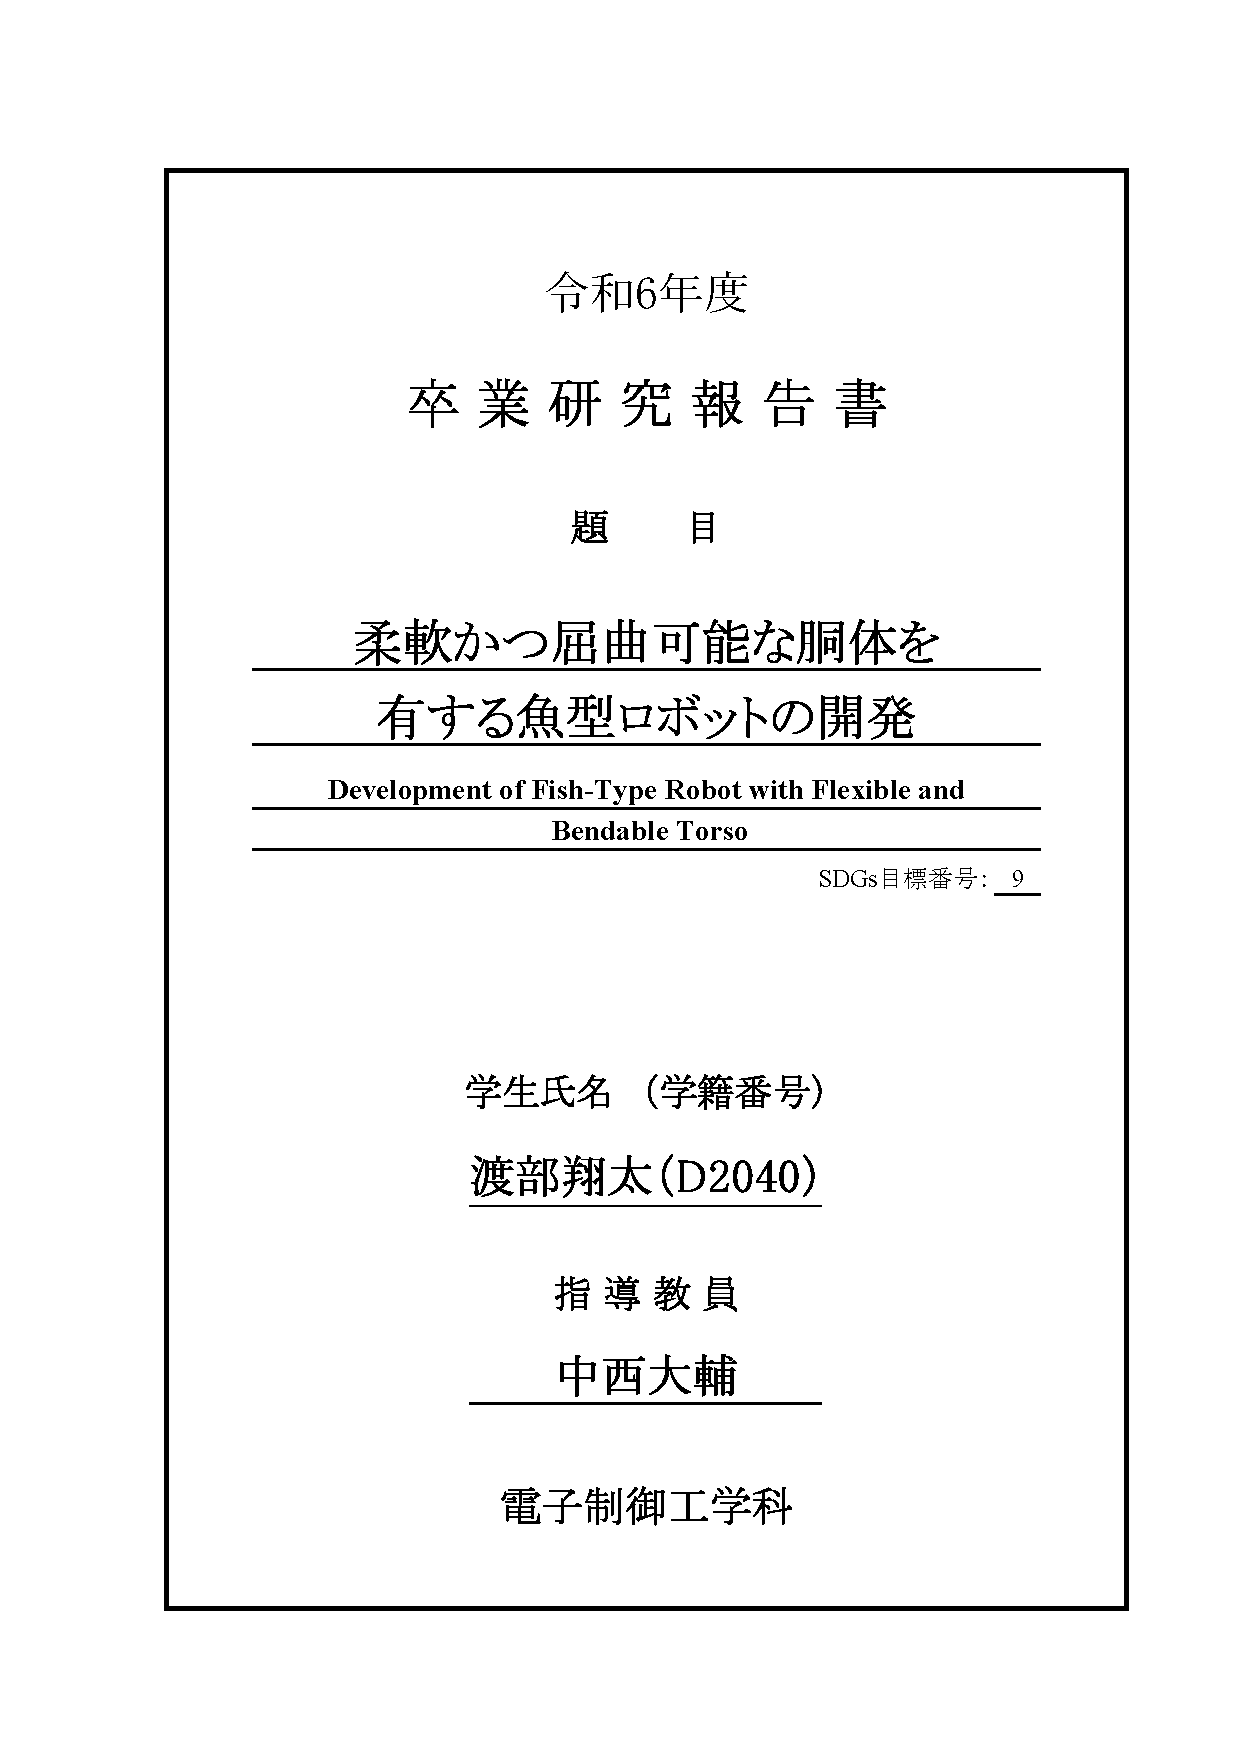
\includepdf[pages=1]{front.pdf}
\thispagestyle{empty}
\newpage
\section*{概要}
水中の推進システムにはスクリュープロペラを用いた推進方法や魚を模したロボットによる尾びれ推進などがあげられる.スクリュープロペラは水上,水中における推進性能が高く,
船舶などに広く用いられている.しかし,生態系調査の面で考えると,スクリュープロペラは周辺環境に影響を与え,調査に適しているとは言えない.その一方で尾びれ推進は周辺環境に影響を与えることがなく,尚且つ加速性・旋回性に優れているため障害物を避けながら目的の地点まで速やかな移動を可能にする.以上のことから水害などの災害支援,水中生物の
生態系調査の面で魚型ロボットの開発は注目されている.そこで我々の研究室ではこれまで様々な魚型ロボットを開発してきた.特に昨年度は魚らしくしなやかな動きを可能にするワイヤ駆動
式の魚ロボットと,完全防水可能かつ魚らしい流線形のボディを有する柔軟外皮装着型の魚ロボットの開発に成功した.しかし,昨年度の先行研究には次のような課題があった.ワイヤ駆動式の
魚ロボットには骨格リンク間にできる隙間に水が入り込み,体全体を使って水をかけないといった課題が,柔軟外皮装着型のロボットには骨格リンクの動きに外皮が追従せず,十分な遊泳性能を
得られなかったという課題があった.そこで本研究ではワイヤ駆動式の魚ロボットに柔軟外皮を装着することによって,魚らしいしなやかな動きを可能にし,かつ骨格リンクの動きに外皮が追従
できるようにすることで十分な遊泳性能を発揮できる魚ロボットを開発した.また,外皮あり・なしそれぞれで直進遊泳実験を行い,外皮による遊泳性能に与える影響について検証を行った.遊
泳実験の結果,外皮を装着することによって遊泳速度が向上することがわかった.速度が向上した要因としては,ロボットのボディが外皮を装着することによって流線形になったことが考えられ
る.したがって流線形のボディを備えることは,遊泳速度を向上させるのに非常に有効であると考えられる.
\newpage
\section*{Abstract}
In underwater propulsion systems, methods such as using screw propellers and fish-like robots with tail fin propulsion are commonly mentioned. Screw propellers 
have high propulsion performance both on the water surface and underwater, and are widely used in ships and other vessels. However, from the perspective of ecosystem 
surveys, screw propellers are not ideal, as they can impact the surrounding environment and are not suitable for surveys. On the other hand, tail fin propulsion 
does not affect the surrounding environment, and its excellent acceleration and maneuverability enable swift movement to a target location while avoiding obstacles. 
For these reasons, the development of fish-like robots has attracted attention for applications in disaster response, such as in the case of flooding, and for aquatic 
ecosystem surveys.
In our laboratory, we have developed various types of fish-like robots. In particular, last year we succeeded in developing a wire-driven fish robot that enables 
flexible movements similar to a real fish, as well as a soft-skin fish robot with a streamlined body and complete waterproofing. However, there were some challenges 
in last year's research. The wire-driven fish robot faced the issue of water entering the gaps between the skeletal links, which prevented efficient water management 
across the entire body. The soft-skin robot encountered the problem that the skin did not follow the movements of the skeletal links, leading to insufficient swimming 
performance.
Therefore, in this study, we developed a fish robot by attaching a soft skin to the wire-driven robot, enabling flexible, fish-like movements while allowing the skin 
to follow the movement of the skeletal links. This development ensures sufficient swimming performance. Additionally, we conducted swimming experiments with and without 
the soft skin to investigate the impact of the soft skin on swimming performance. The results of these experiments showed that the swimming speed increased when the soft 
skin was attached. The increase in speed is believed to be due to the streamlined body shape achieved by the soft skin. Hence, it can be concluded that having a streamlined 
body is highly effective in improving swimming speed.
        % 概要
\thispagestyle{empty}
\newpage
\section*{Abstract}
Underwater propulsion systems include screw propeller propulsion and tail fin propulsion using fish-like robots. Screw propellers provide high propulsion efficiency 
both in the water and underwater, and they are widely used in ships and other vessels. However, from an ecosystem research perspective, screw propellers can affect 
the surrounding environment and are not ideal for surveys. On the other hand, tail fin propulsion has less environmental impact and offers excellent acceleration 
and maneuverability, enabling rapid movement toward a target while avoiding obstacles. These advantages make it well-suited for disaster relief, such as in flooding, 
as well as for studying the ecosystems of underwater organisms.
As a result, the development of fish-shaped robots has gained attention for both disaster support and underwater ecosystem research. In our laboratory, we have developed 
various fish-shaped robots. Specifically, last year, we successfully developed a wire-driven fish robot that enables supple, fish-like movements, as well as a waterproof 
fish robot with a streamlined, fish-like body and flexible outer skin. However, the wire-driven system had gaps between the links, meaning water could not be splashed off
 the body. In the flexible skin model, the skeletal links and skin were not synchronized, resulting in limited movement of the body.
In this study, we combined these two approaches to develop a wire-driven fish-shaped robot with a flexible outer skin. This innovation allows for supple, fish-like movement 
while also enabling the robot to splash water off its torso, thus improving swimming performance. The swimming experiments confirmed that the wire-driven system achieved
 fish-like movements, with the flexible outer skin moving in accordance with the link movements. Additionally, we conducted straight-line swimming experiments with and 
 without the outer skin to assess its impact on swimming performance. The results showed that the swimming speed increased when the outer skin was attached. This increase 
 in speed is likely due to the robot’s body becoming more streamlined when the skin was added. Therefore, having a streamlined body is highly effective in improving swimming 
 speed.

\thispagestyle{empty}
\newpage
\tableofcontents
\thispagestyle{empty}

%章ごとに呼び出し

\newpage
\setcounter{page}{1}
\section{緒言}
水中の推進システムにはスクリュープロペラを用いた推進方法や魚を模したロボットによる尾びれ推進などがあげられる\cite{ichi}.スクリュープロペラは水上,水中における推進性能が高く,
船舶などに広く用いられている.しかし,生態系調査の面で考えると,スクリュープロペラは周辺の植物や水中動物などを巻き込んで水中の環境に影響を与え,騒音によって周辺生物を
驚かせるなど,調査に適しているとは言えない.その一方で尾びれ推進は周辺生物を巻き込むなど環境に影響を与えにくく,尚且つ加速性・旋回性に優れているため障害物を避けながら
目的の地点まで高機動な遊泳を可能にする.以上のことから水害などの災害支援,水中生物の生態系調査の面で魚型ロボットの開発は注目されている\cite{ni}\cite{san}.

そこで我々の研究室ではこれまで様々な魚型ロボットを開発してきた.駆動機構として弾性体を用いた飛び移り座屈機構を採用した魚ロボット\cite{yon}\cite{go}や,それに加えて屈曲可能な胴体
構造を有する魚ロボット\cite{roku,nana,hachi}の開発に成功してきた.さらに昨年度卒業研究では駆動機構としてワイヤ駆動方式を用いたより魚らしい形状を持つ魚ロボットの開発に成功し,
魚のように胴体を屈曲させてしなやかに遊泳を行うことができた.しかし,これらの魚ロボットには弾性体に追従する骨格リンクの隙間に水が入り込み,結果的に弾性体のみで水をかいてしまい,体全体でかく
ことができていないという課題があった.

一方で同じく昨年度卒業研究(先行研究\cite{kyu})ではこの課題を解決するために,胴体部全体をシリコン製の柔軟外皮で覆った魚型ロボットの開発が行われた.柔軟外皮は魚らしい流線型のフォルムの実現のみならず,従来のOリングを
用いた手法よりも容易かつ確実性の高い防水性能を実現した.しかし,遊泳に関しては骨格リンクの動きに柔軟外皮が追従せず,胴体部を振って泳ぐことはできなかった.そのため遊泳速度が大きく低下し,柔軟
外皮が遊泳速度に対してどのように影響を与えるのか検証することができなかった.

そこで本研究では,しなやかな遊泳が可能なワイヤ駆動方式と,流線形の胴体フォルムを実現可能な柔軟外皮を組み合わせた魚型ロボットを開発する.ロボットはアジのスキャンデータを基に作成し,アジ型遊泳の定義\cite{juu}のもとに,
胴体後ろ半分を屈曲させることで遊泳を行う.そして柔軟外皮あり・なしで直進遊泳実験を行い,柔軟外皮が遊泳性能に与える影響について検証・考察を行う.
    % 緒言
\newpage
\section{先行研究}
本章では,本研究で開発したロボットのベースとなった機体を先行研究を用いて述べ,それぞれの実験結果とそこから得られた知見をまとめる.

\subsection{柔軟外皮装着型魚ロボット}
先行研究\cite{kyu}で開発された機体を図\ref{fig:robot_sen}\cite{kyu}に,構造を図\ref{fig:kouzou_sen}\cite{kyu}に示す.先行研究\cite{kyu}ではハマチをモデルにしてロボットを作製していた.
図\ref{fig:migaihi_sen}は魚型ロボットに柔軟外皮を取り付けたものであり,水中に沈めること及び水中での姿勢維持を目的として,柔軟外皮を固定する防水リングにおもりが取り付けてある.おもり
の重さは頭部と尾びれ部分でそれぞれ296 g,150 gである.本機体は全長477 mm,重さ1080 g,おもりを含めた重さが1526 gとなっている.本機体は頭部と胴体部の大きく二つに分けることができる.

\begin{figure}[htbp]
    \centering
    \begin{tabular}{cc}
     \begin{minipage}[b]{0.45\linewidth}
        \centering
        \setPicture{zenrarobot.jpg}
        \subcaption{外皮未装着時}
        \label{fig:gaihi_sen}
     \end{minipage}
     \hspace{0.05\linewidth}
     \begin{minipage}[b]{0.45\linewidth}
        \centering
        \setPicture{fishrobot.jpg}
        \subcaption{外皮装着時}
        \label{fig:migaihi_sen}
     \end{minipage}
    \end{tabular}
    \caption{柔軟外皮装着型の魚ロボット\cite{kyu}}
    \label{fig:robot_sen}
\end{figure}
\begin{figure}[b]
    \centering
    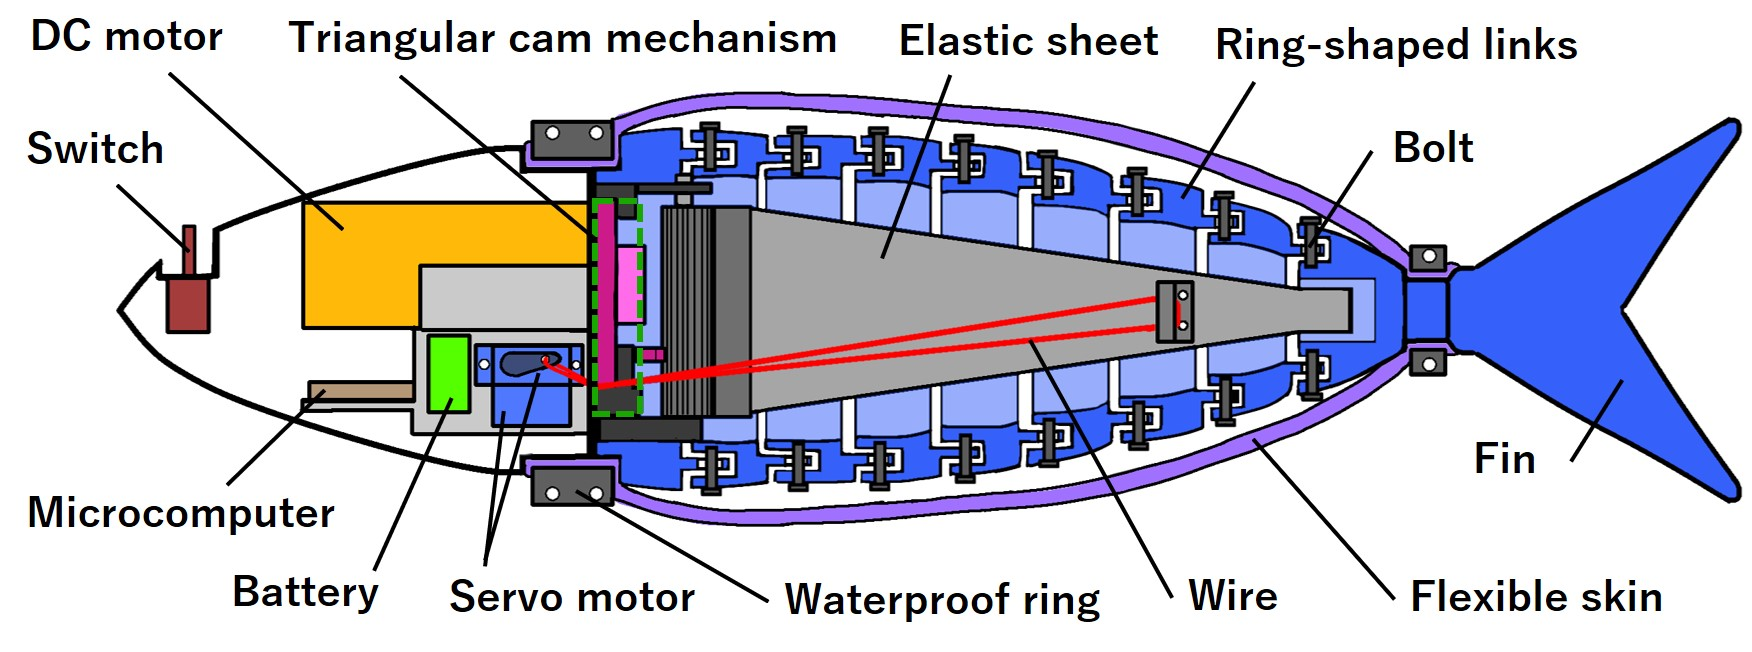
\includegraphics[width=1\linewidth]{chapters/picture/mosikizu.jpg}
    \caption{ロボットの構造\cite{kyu}}
    \label{fig:kouzou_sen}
\end{figure}

\subsubsection{頭部}
本機体の頭部には,DC モータ( タミヤ社,AO-8033),サーボモータ(Tower Pro 社,MG92B)二つ,マイコン(M5Stack Technology 社,M5STACK-K051),モータ用Lipo バッ
テリ(Hyperion 社,G5 50Cmax 7.4 V-240 mAh),マイコン用Lipo バッテリ(DATA POWERTECHNOLOGY 社,DTP502535),スイッチが入っている.モータは頭部に収まるものの中
でなるべくトルクの強いものが用いられている.また,上に挙げたスイッチ以外の部品はすべて頭部の外殻ではなく内側のふたに取り付けられている.

\begin{figure}[t]
    \centering
     \begin{minipage}[b]{0.45\linewidth}
        \centering
        \setPicture{zakutu1.png}
        \caption{飛び移り座屈発生機構の模式図\cite{kyu}}
        \label{fig:zakutu1_sen}
     \end{minipage}
     \begin{minipage}[b]{0.35\linewidth}
        \centering
        \setPicture{zakutu2.png}
        \caption{たわみ長さの定義\cite{kyu}}
        \label{fig:zakutu2_sen}
     \end{minipage}
     \begin{minipage}[b]{0.15\linewidth}
        \centering
        \setPicture{link.png}
        \caption{関節の構造\cite{kyu}}
        \label{fig:kansetu}
     \end{minipage}
\end{figure}

\subsubsection{胴体部}
まず,先行研究\cite{kyu}で駆動機構として用いられた飛び移り座屈について記す.飛び移り座屈とは,弾性を有する柔軟体の変形によって発生する連続的な現象であり,
瞬間的に大きな力を発生させることができる.先行研究ではサーボモータを用いて弾性体をたわませ,DCモータを用いて弾性体を変形させることで飛び移り座屈を
発生させている.ここで実験に用いる語句とパラメータを定義する.図\ref{fig:zakutu1_sen}に飛び移り座屈発生機構の模式図を示す.弾性体の自然長を$l$,弾性体をたわませた際の軸間
距離を$L$,弾性体がどの程度たわんでいるかを示すたわみ長さを$d$として,たわみ長さを$d=l−L$と定義する.

次に胴体部について,胴体部は屈曲可能な8関節9リンク構造になっており,リンクの接続部は図\ref{fig:kansetu}のようにベアリング(内径3 mm)とボルト(M2)で接続されている.
また,すべてのリンクで合計$90\:^\circ$曲げるため一関節あたり$11.25\:^\circ$曲がるよう設計されている.$90\:^\circ$という値は,実際のハマチの動く様子から決定している.
なお,各リンクには機体を水中に沈めるために板おもり(22 g)を合計10 枚張り付けてある.次に,飛び移り座屈に用いる弾性体について記す.ここでの弾性体とは外力により曲がる薄
い板のことを指す.先行研究では0.2 mm厚のステンレス(岩田製作所,SUS02)に加え,弾性を強めるために1 mm厚のポリプロピレン(セイワ・プロ社,23-589)を貼り合わせたものを使用している.

\subsection{遊泳実験}
\subsubsection{実験条件}
直進遊泳をさせるため,サーボモータを$90\:^\circ$回し,たわみ長さを10 mmに固定した.その上でDCモータに印加する電圧を1.5 V,2.0 V,2.5 Vに変化させて遊泳を行っ
た.また,機体内部に防水シールを貼り,遊泳時においても防水ができているか確認する.



\subsubsection{実験結果}
印加電圧1.5 V時の遊泳の様子を図\ref{fig:swim_sen}に示す.遊泳には成功したが,遊泳の軌道が少し曲がってしまっていることがわかる.また,印加電圧と遊泳速度の関係を図\ref{fig:speed}に示す.
電圧が大きくなるにつれて,遊泳速度も大きくなっていることがわかる.本機体の最高遊泳速度は印加電圧2.5 V時の43 mm/sであった.
直進遊泳をするはずが少し曲がってしまったことについて,これは,弾性体をたわませる二つの糸の長さが異なることが原因として考えられる.弾性体をたわませ
る力が左右で違ったことにより飛び移り座屈で発生する力にも左右で差が出てしまうので,結果曲がってしまったと考えられる.
次に遊泳速度が遅い原因として2 つ考えられる.1 つ目はたわみ長さが小さかったことである.たわみ長さや尾びれの振れ角が大きい程飛び移り座屈を発生させたときに放出する
力は大きくなるが,飛び移り座屈を発生させるために必要な力も大きくなる.また2 つ目の原因として,外皮とリンクの間に余分な隙間があったため,リンクの動きを外皮に伝えることができな
かったということが考えられる.
\begin{figure}[htbp]
    \centering
    \begin{minipage}[b]{0.5\linewidth}
        \centering
        \setPicture{swim.png}
        \caption{遊泳実験の様子\cite{kyu}}
        \label{fig:swim_sen}  
    \end{minipage}
    \hspace{0.05\linewidth}
    \begin{minipage}[b]{0.4\linewidth}
        \centering
        \setPicture{speed.eps}
        \caption{印加電圧と遊泳速度の関係\cite{kyu}}
        \label{fig:speed}  
    \end{minipage} 
\end{figure}
\begin{figure}[b]
    \centering
    \begin{tabular}{ccc}
        \begin{minipage}[b]{0.3\linewidth}
            \centering
            \setPicture{aka.png}
            \subcaption{赤く染まった防水シール}
            \label{fig:aka_sen}
        \end{minipage}
        \begin{minipage}[b]{0.3\linewidth}
            \centering
            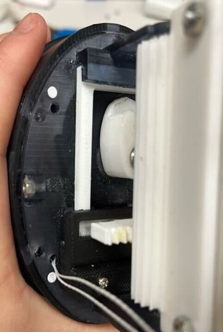
\includegraphics[width=0.6\linewidth]{chapters/picture/siro_naka.png}
            \subcaption{機体内部の防水シール}
            \label{fig:naka_sen}
        \end{minipage}
        \begin{minipage}[b]{0.3\linewidth}
            \centering
            \setPicture{siro_obire.png}
            \subcaption{尾びれ側の防水シール}
            \label{fig:obire_sen}
        \end{minipage}
    \end{tabular}
    \caption{遊泳実験後の防水シールの様子\cite{kyu}}
    \label{fig:bousui_sen}
\end{figure}
遊泳実験を行った後機体を開けてみると,防水シールはわずかに染まった一か所を除いてすべて白いままであった(図\ref{fig:bousui_sen}).このことから,機体内部の防水に成功したことが分かる.

\subsection{得られた知見}
先行研究では柔軟外皮を開発し,柔軟外皮を用いての完全防水に成功した.しかし,柔軟外皮と骨格リンクに隙間ができてしまい,リンクの動きに柔軟外皮を追従させることができなかった.柔軟外皮をリンクに密着
させる,または柔軟外皮とリンクを追従させるための構造を開発することによってリンクの動きを柔軟外皮に伝えることが可能だと考えられる.また,柔軟外皮を用いて胴体部に防水を行っていたため,胴体が浮袋に
なり重りを多く付ける必要があった.これについては胴体部を柔軟外皮で包んだ上で中に水を入れて浸水させることで,遊泳姿勢を重りを使わずに安定させることができると考える.            % 本文
\newpage
\section{柔軟外皮を備えたワイヤ駆動式魚ロボットの開発}
前章で述べたように,先行研究\cite{kyu}では屈曲可能な胴体を持ち,柔軟外皮を装着して完全防水を可能にした魚ロボットの開発に成功した.しかし,リンクと外皮に隙間ができてしまい,
リンクの動きを外皮にうまく伝えることができなかった.そこで本研究では魚らしいしなやかな動きを可能にするワイヤ駆動式の魚ロボットをベースにリンクに外皮を追従させ,尾びれのみならず
胴体部まで振って泳ぐことが可能なロボットの開発を目指す.本章ではその予備的な開発として,昨年度卒業研究を参考に外皮を持たないワイヤ駆動式魚型ロボットを開発し,柔軟外皮をどのよう
に組み合わせるべきかなどについて検討を行う.
\subsection{ワイヤ駆動式魚型ロボットの動作原理}
昨年度卒業研究で提案され,本研究でも採用したワイヤ駆動の動作原理を記す.ロボット前方にはプーリを取り付けたサーボモータを配置し,胴体部には弾性体とそれに固定した骨格リンクを配置する.
ワイヤはプーリーから骨格リンクに設けられた穴を通って尾びれ付け根まで伸びており,プーリーを回してワイヤを巻き取ることによって弾性体が曲がり,胴体部を屈曲させることができる.それを左
右に繰り返すことで遊泳を可能にする(図\ref{fig:waiyakudou}).

\begin{figure}[b]
   \centering
   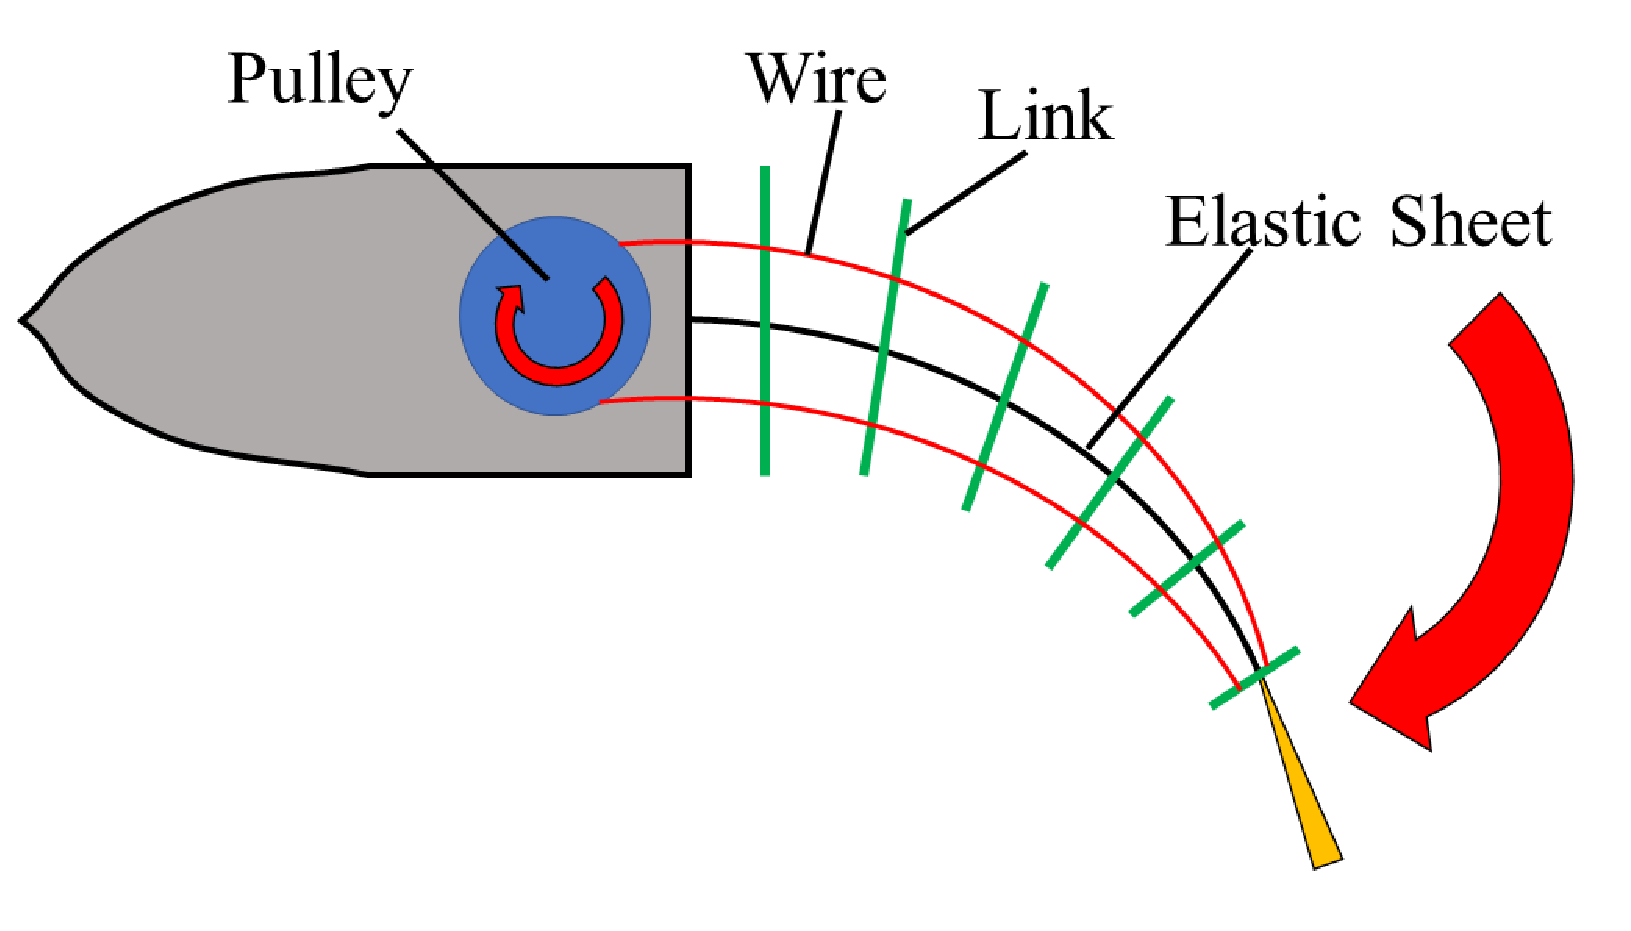
\includegraphics[width=0.6\linewidth]{chapters/picture/waiyakudou.eps}
   \caption{ワイヤ駆動のイメージ}
   \label{fig:waiyakudou}
\end{figure}

\subsection{試作機}
\subsubsection{試作機の作製}
まず,昨年度卒業研究を参考にして試作機を作製した.図\ref{fig:sisaku}に外観を,図\ref{fig:kouzou_sisaku}に構造を示す.全長は530 mm,重量は478 gである.試作機は頭部と胴体部の二つ
の部分で構成している.

頭部には制御回路とバッテリーを搭載しており,えらにあたる部分には防水仕様(IP67)の サーボモータ(Flash Hobby, M45CHW)を配置している.サーボモータは270°回転できるようになっている.
使用マイコンはM5Stamp Pico(M5Stack Technology 社),使用バッテリーはマイコン用の3.7 V,サーボモータ用の7.4 Vの二つのLi-ionバッテリーを使用している.そのため,頭部は防水が必要となり,
頭部の断面にOリングをはめ込むことによって防水を行っている.頭部はネジ穴が空いたものと,ナット用の穴が空いたものに分かれており,これらはM1.7ネジで固定される.
胴体部は骨格リンク(PLA樹脂)と弾性体(ポリプロピレン板,厚さ0.75 mm),尾びれ(TPU樹脂,厚さ2 mm)で構成されており,骨格リンクは図のように楕円形にして作製し,ワイヤ(ポリエステル製,0.40 mm)
を通す穴を空けている.

\begin{figure}[t]
    \centering
    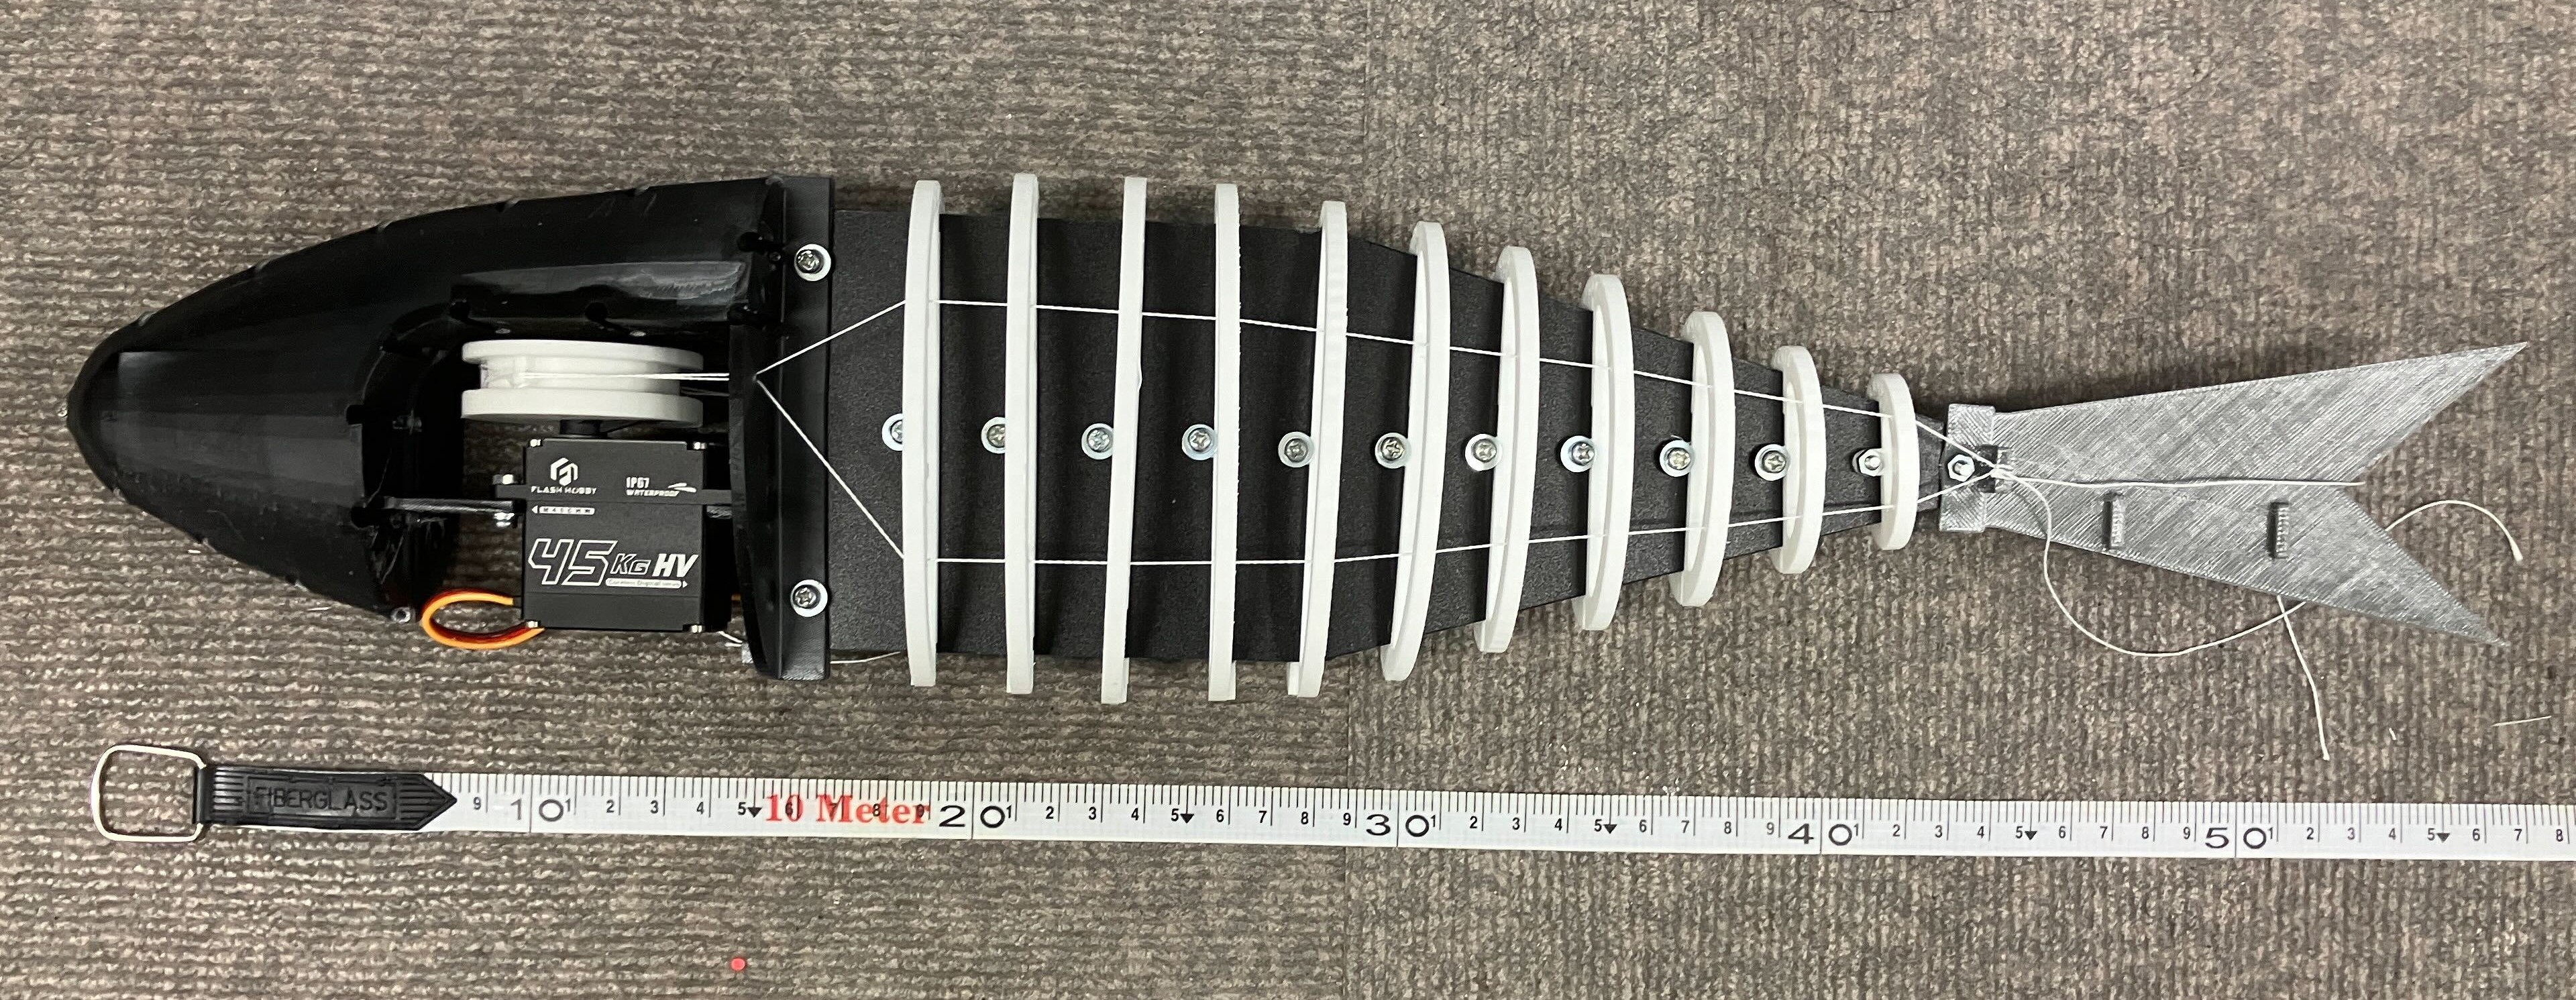
\includegraphics[width=0.80\linewidth]{chapters/picture/sisaku.jpg}
    \caption{試作機の外観}
    \label{fig:sisaku}
\end{figure}
\begin{figure}[t]
    \centering
    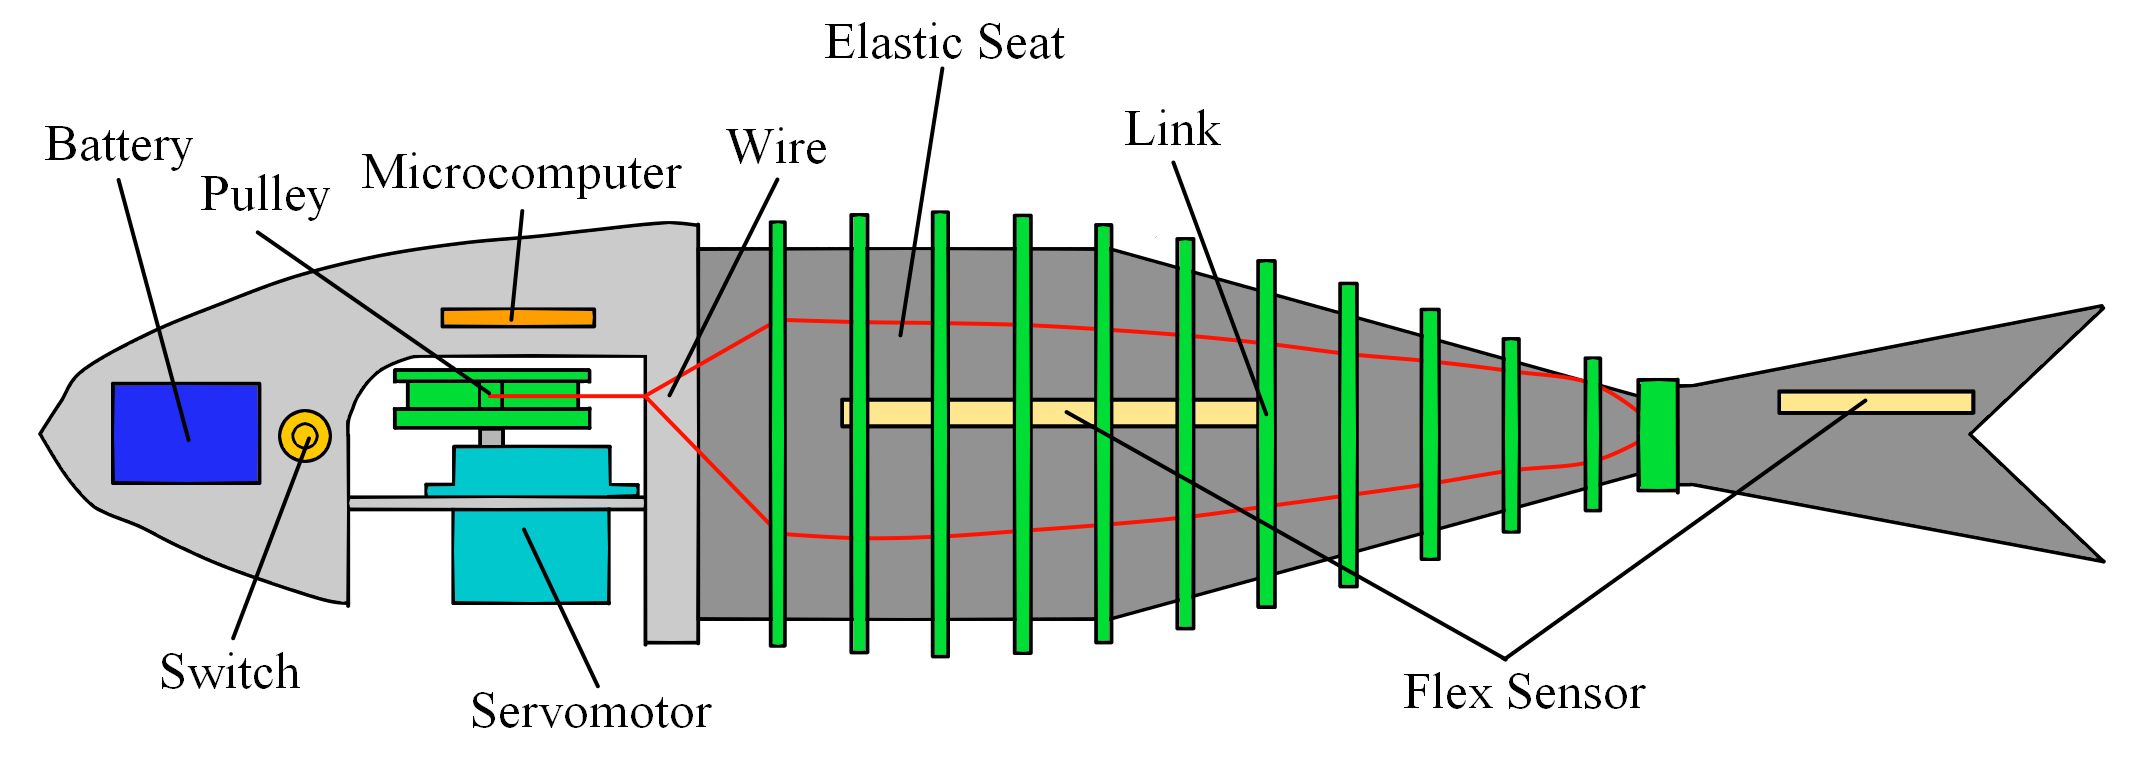
\includegraphics[width=0.80\linewidth]{chapters/picture/tentativeschematic.png}
    \caption{試作機の構造}
    \label{fig:kouzou_sisaku}
\end{figure}
\begin{figure}[t]
    \centering
     \begin{minipage}[b]{0.50\linewidth}
        \centering
        \setPicture{ring.jpg}
        \caption{頭部断面のようす}
        \label{fig:danmen}
     \end{minipage}
     \hspace{0.05\linewidth}
     \begin{minipage}[b]{0.25\linewidth}
        \centering
        \setPicture{jikkilink.png}
        \caption{骨格リンク}
        \label{fig:link_sen}
     \end{minipage}
\end{figure}

\subsubsection{防水テスト・遊泳テスト}
機体完成後,防水テストと遊泳テストを行った.まず防水テストは水没すると赤くなるシールを頭部内部に貼り,水深120 mmの水槽で2 分間沈める防水テストを7回行った.それぞれねじの締め具合や
頭部の歪みを直しながらテストをしたが,完全な防水はできず,7回目で頭部下方のみの浸水にとどまったのでこれで防水できていると判断した(図\ref{fig:bousuitest_sisaku}).
次に遊泳テストを行った.遊泳テストの様子を図\ref{fig:test_sisaku}に示す.

\begin{figure}[t]
    \centering
    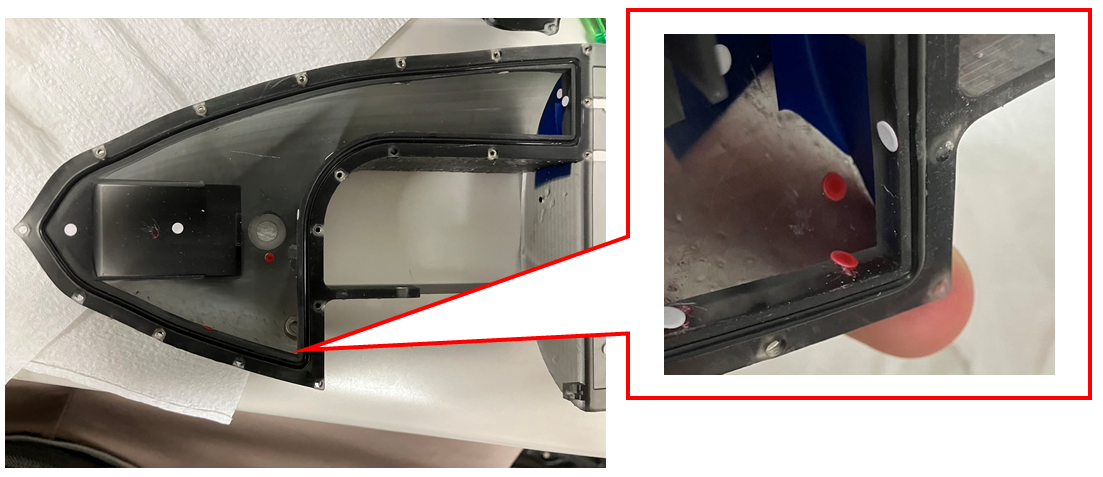
\includegraphics[width=0.80\linewidth]{chapters/picture/bousuitest.png}
    \caption{頭部下方浸水のようす}
    \label{fig:bousuitest_sisaku}
\end{figure}
\begin{figure}[t]
    \centering
    \setPicture{sisakuoyogu2.png}
    \caption{遊泳テストの様子}
    \label{fig:test_sisaku}
\end{figure}

\subsubsection{試作機から得られた知見}
試作機の作製・動作確認を通して得られた知見として,まず,頭部をネジとOリングを用いて防水する方法は完全な防水に至らないと考えられる.また,頭部を固定するネジが多いと,バッテリー交換が
しにくく,メンテナンス性が悪くなるということも分かった.以上のことから防水方法を変更し,メンテナンス性を向上させた頭部に改良することが必要だと考える.そこで防水を比較的容易な方法ででき,
完全防水可能な柔軟外皮を用いて頭部の防水を行うようにする.また,骨格リンクが胴体の形状をなしていることを生かし,骨格リンクをはめられるような溝を胴体外皮内部に作製することでリンクと
外皮の追従を行う.
\newpage

\section{柔軟外皮装着型ワイヤ駆動式魚ロボット}
本章では先行研究\cite{kyu}や試作ロボットから得られた知見をもとに開発した,柔軟外皮とリンクが連動し,完全防水可能かつメンテンナンス性を向上させた柔軟外皮装着型
のワイヤ駆動式魚ロボットについて述べる.
\subsection{ロボット概要}
図\ref{fig:gaikan}に開発したロボットを示す.開発した魚ロボットは体長470 mm,重量は重り(25 g)を含めて710 gである.
\begin{figure}[htbp]
    \centering  
    \begin{subfigure}[b]{0.85\linewidth}
        \centering
        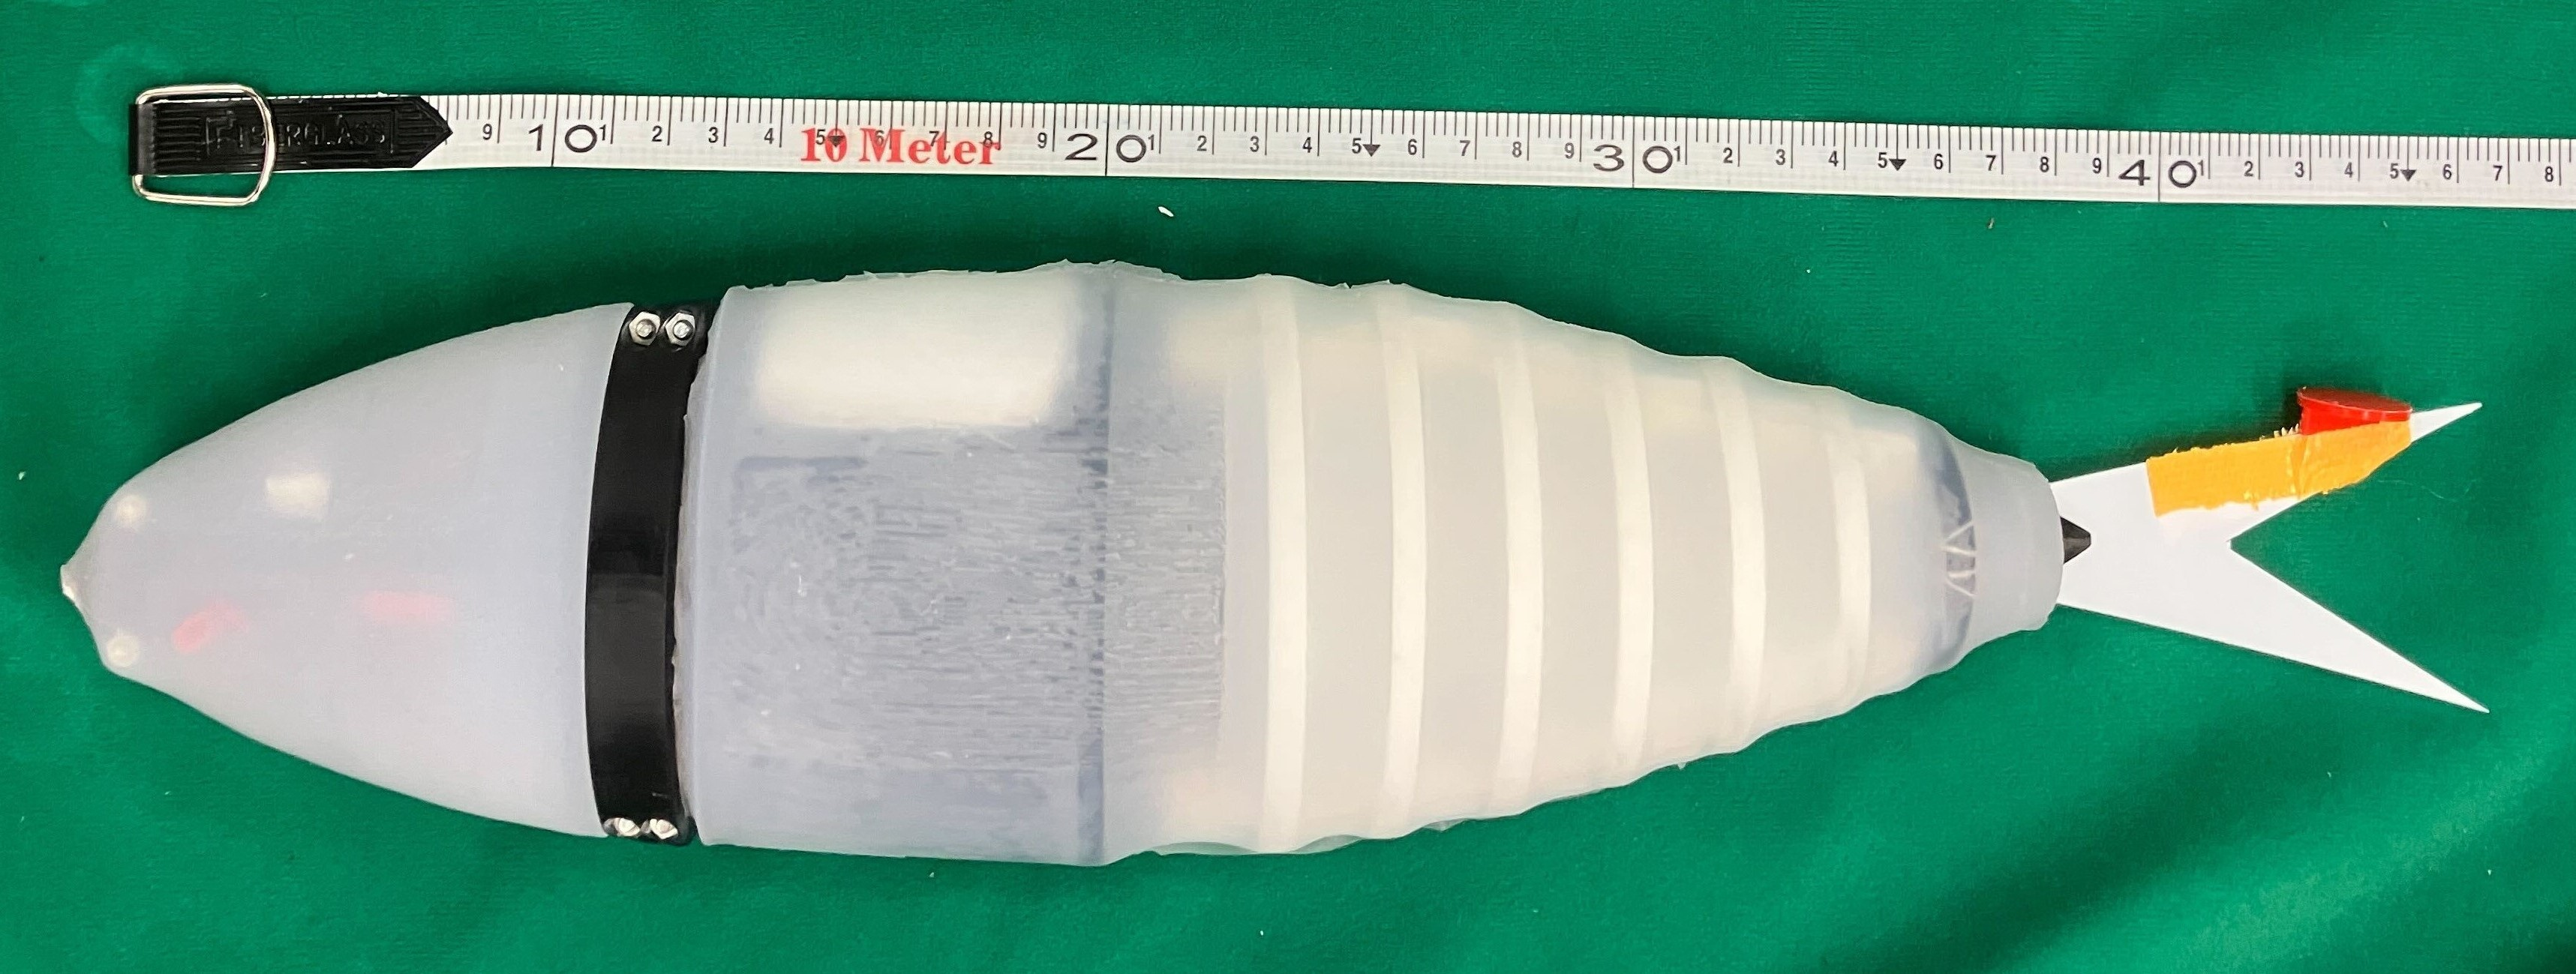
\includegraphics[width=0.9\linewidth]{chapters/picture/withskin.jpg}
        \subcaption{柔軟外皮装着時}
        \label{fig:fishrobo_with}
    \end{subfigure}
    \begin{subfigure}[b]{0.85\linewidth}
        \centering
        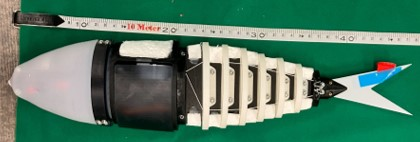
\includegraphics[width=0.9\linewidth]{chapters/picture/without_skin.jpg}
        \subcaption{胴体部の柔軟外皮未装着時}
        \label{fig:fishrobo_less}
    \end{subfigure}
    \begin{subfigure}[b]{0.85\linewidth}
        \centering
        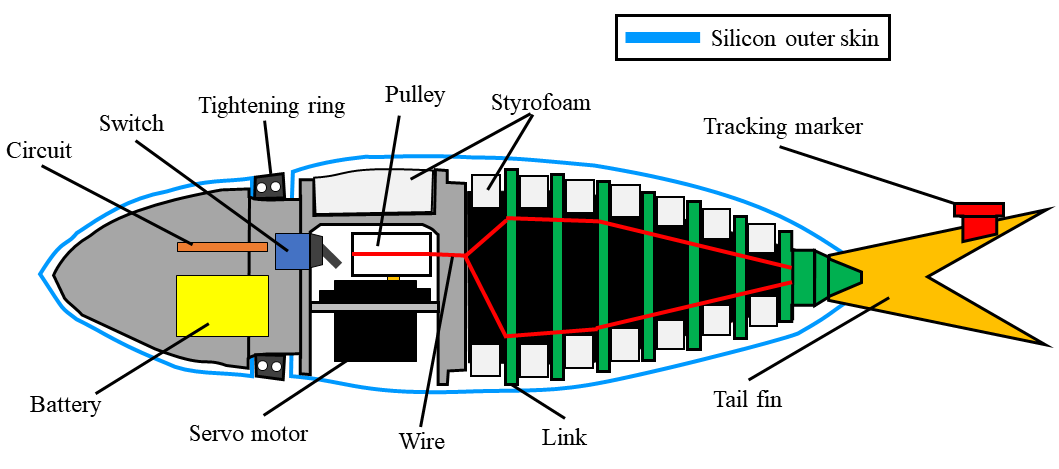
\includegraphics[width=0.9\linewidth]{chapters/picture/fish.png}
        \caption{開発したロボットの構造}
        \label{fig:kouzou}
    \end{subfigure}
    \caption{開発した柔軟外皮装着型ワイヤ駆動式魚ロボット}
    \label{fig:gaikan}
\end{figure}
ロボットの外形は
昨年度卒業研究においてアジのスキャンデータ(図\ref{fig:data_scan})から作製したモデルデータ(図\ref{fig:data_model})をもとに作製し,サイズは2倍とした.本機体は頭部・胴体
部・外皮の3つからなり,頭部と胴体部をそれぞれ別の柔軟外皮で包む構造になっている.また,頭部は防水区画とし,胴体部は水中姿勢を水平にするために浸水させた.

\begin{figure}[t]
    \centering
    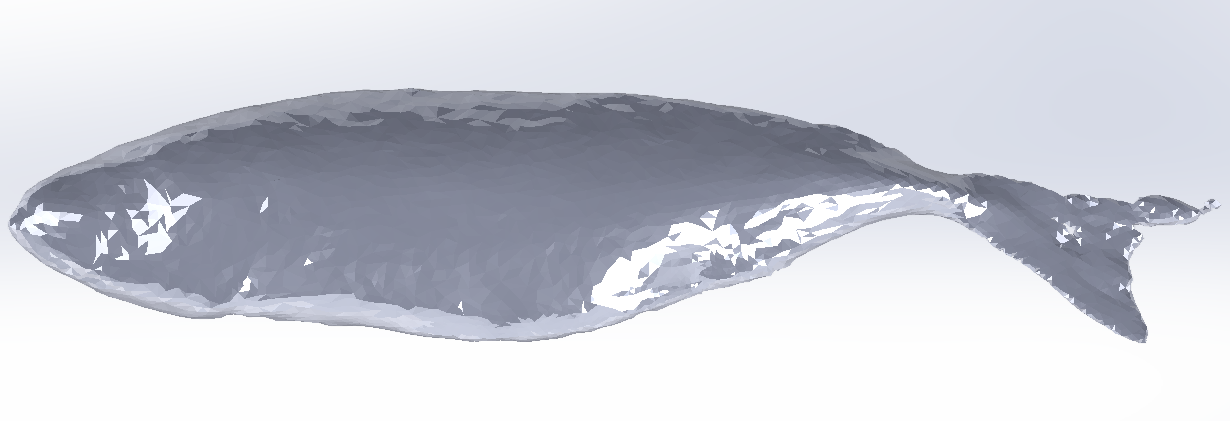
\includegraphics[width=0.7\linewidth]{chapters/picture/scan.png}
    \caption{アジの3Dスキャンデータ}
    \label{fig:data_scan}
\end{figure}
\begin{figure}[t]
    \centering
    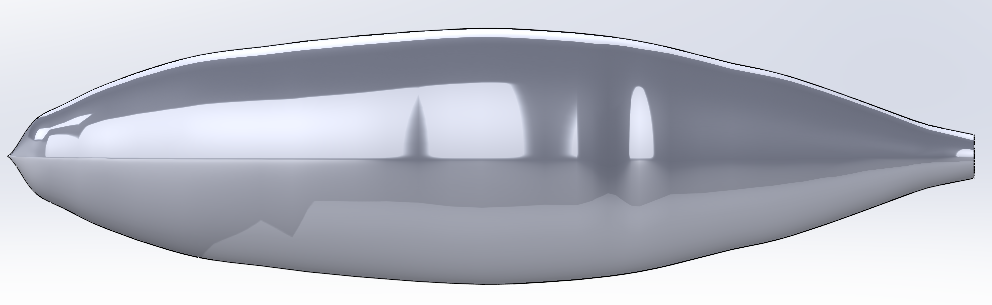
\includegraphics[width=0.7\linewidth]{chapters/picture/fishkinji2.png}
    \caption{アジの3Dモデルデータ}
    \label{fig:data_model}
\end{figure}

\subsection{頭部}
頭部はフレーム部分とシリコン製の外皮部分からなる.フレーム部分は光造形方式の3Dプリンタで作製しており,胴体前部と一体となっている.フレーム内部にはバッテリーと制御回路を搭載しており,使用するバッテリー,マイコン共に試作機と同じものを用いた.バッテリーと
マイコンを搭載する都合上頭部を防水する必要があり,試作機から得た知見をもとに今回はOリングによる防水ではなく,シリコン製の柔軟外皮を用いて防水を行った.
防水方法としてはシリコン製の柔軟外皮を頭部にかぶせ,根元を防水リングによって締め付けることで防水を行った(図\ref{fig:bousui}).防水リングのサイズは文献\cite{juuiti}を参考に締め付ける部分が
短径,長径ともに10%つぶせるように設計した.
また,試作機と同様に防水実験を1回行ったが,内部に貼ったシールはどれも赤く染まらず,完全な防水ができた(図\ref{fig:bousui_test}).
また,フレーム部分は上部と下部のカバーが開くようになっており,メンテナンス性向上のためにねじ止めではなくワンタッチでカバーを開閉できるようにしている
(図\ref{fig:head_open},\ref{fig:rock}).
それに加えて制御回路とバッテリーを取り出しやすくするためにねじで固定するのではなく,図\ref{fig:toubu_kiban},図\ref{fig:toubu_battery}のように溝にはめストッパーをつける
ことで頭部に配置している.

\begin{figure}[t]
    \centering
    \begin{tabular}{cc}
        \begin{minipage}[b]{0.33\linewidth}
            \centering
            \setPicture{bousui.pdf}
            \subcaption{防水構造}
            \label{fig:bousui_kouzou} 
        \end{minipage}
        \begin{minipage}[b]{0.33\linewidth}
            \centering
            \setPicture{jissai.jpg}
            \subcaption{実際に装着した様子}
            \label{fig:bousui_jissai} 
        \end{minipage}
    \end{tabular}
    \caption{頭部防水}
    \label{fig:bousui}
\end{figure}
\begin{figure}[t]
    \centering
    \begin{tabular}{ccc}
        \begin{minipage}[b]{0.25\linewidth}
            \centering
            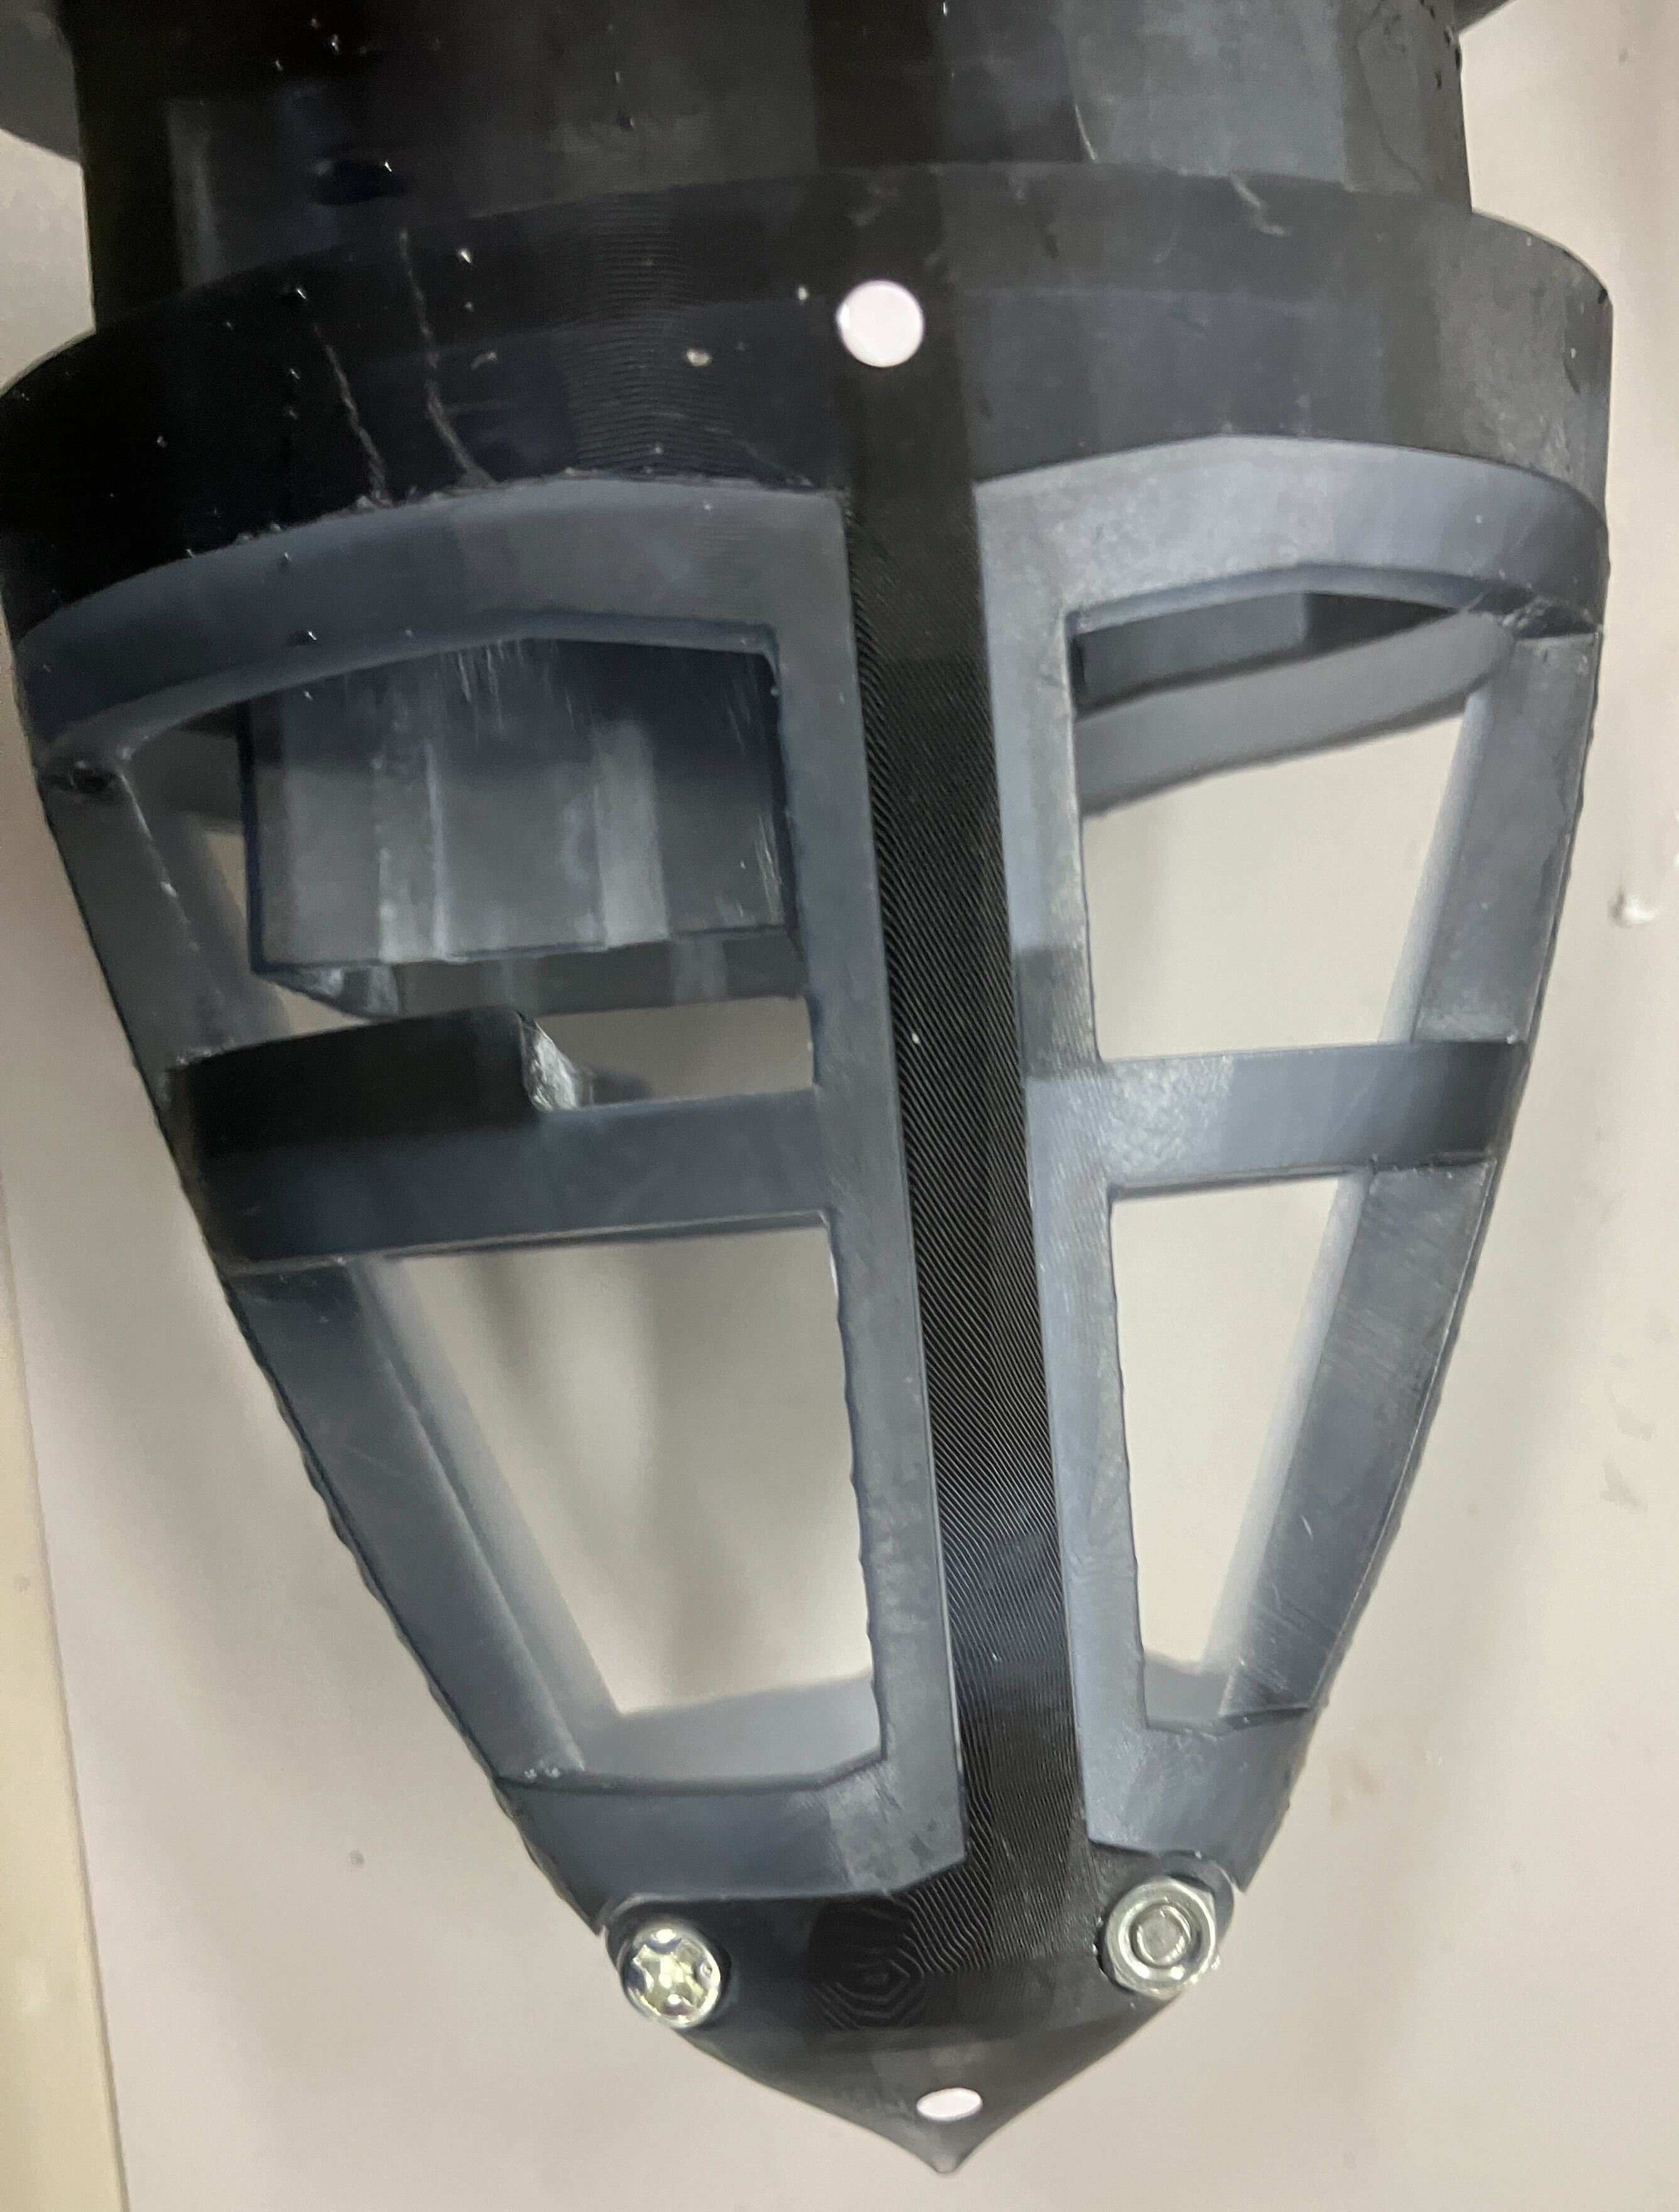
\includegraphics[width=0.7\linewidth]{chapters/picture/bousui_soku.jpg}
            \subcaption{頭部側面}
            \label{fig:toubu_soku}
        \end{minipage}
        \begin{minipage}[b]{0.25\linewidth}
            \centering
            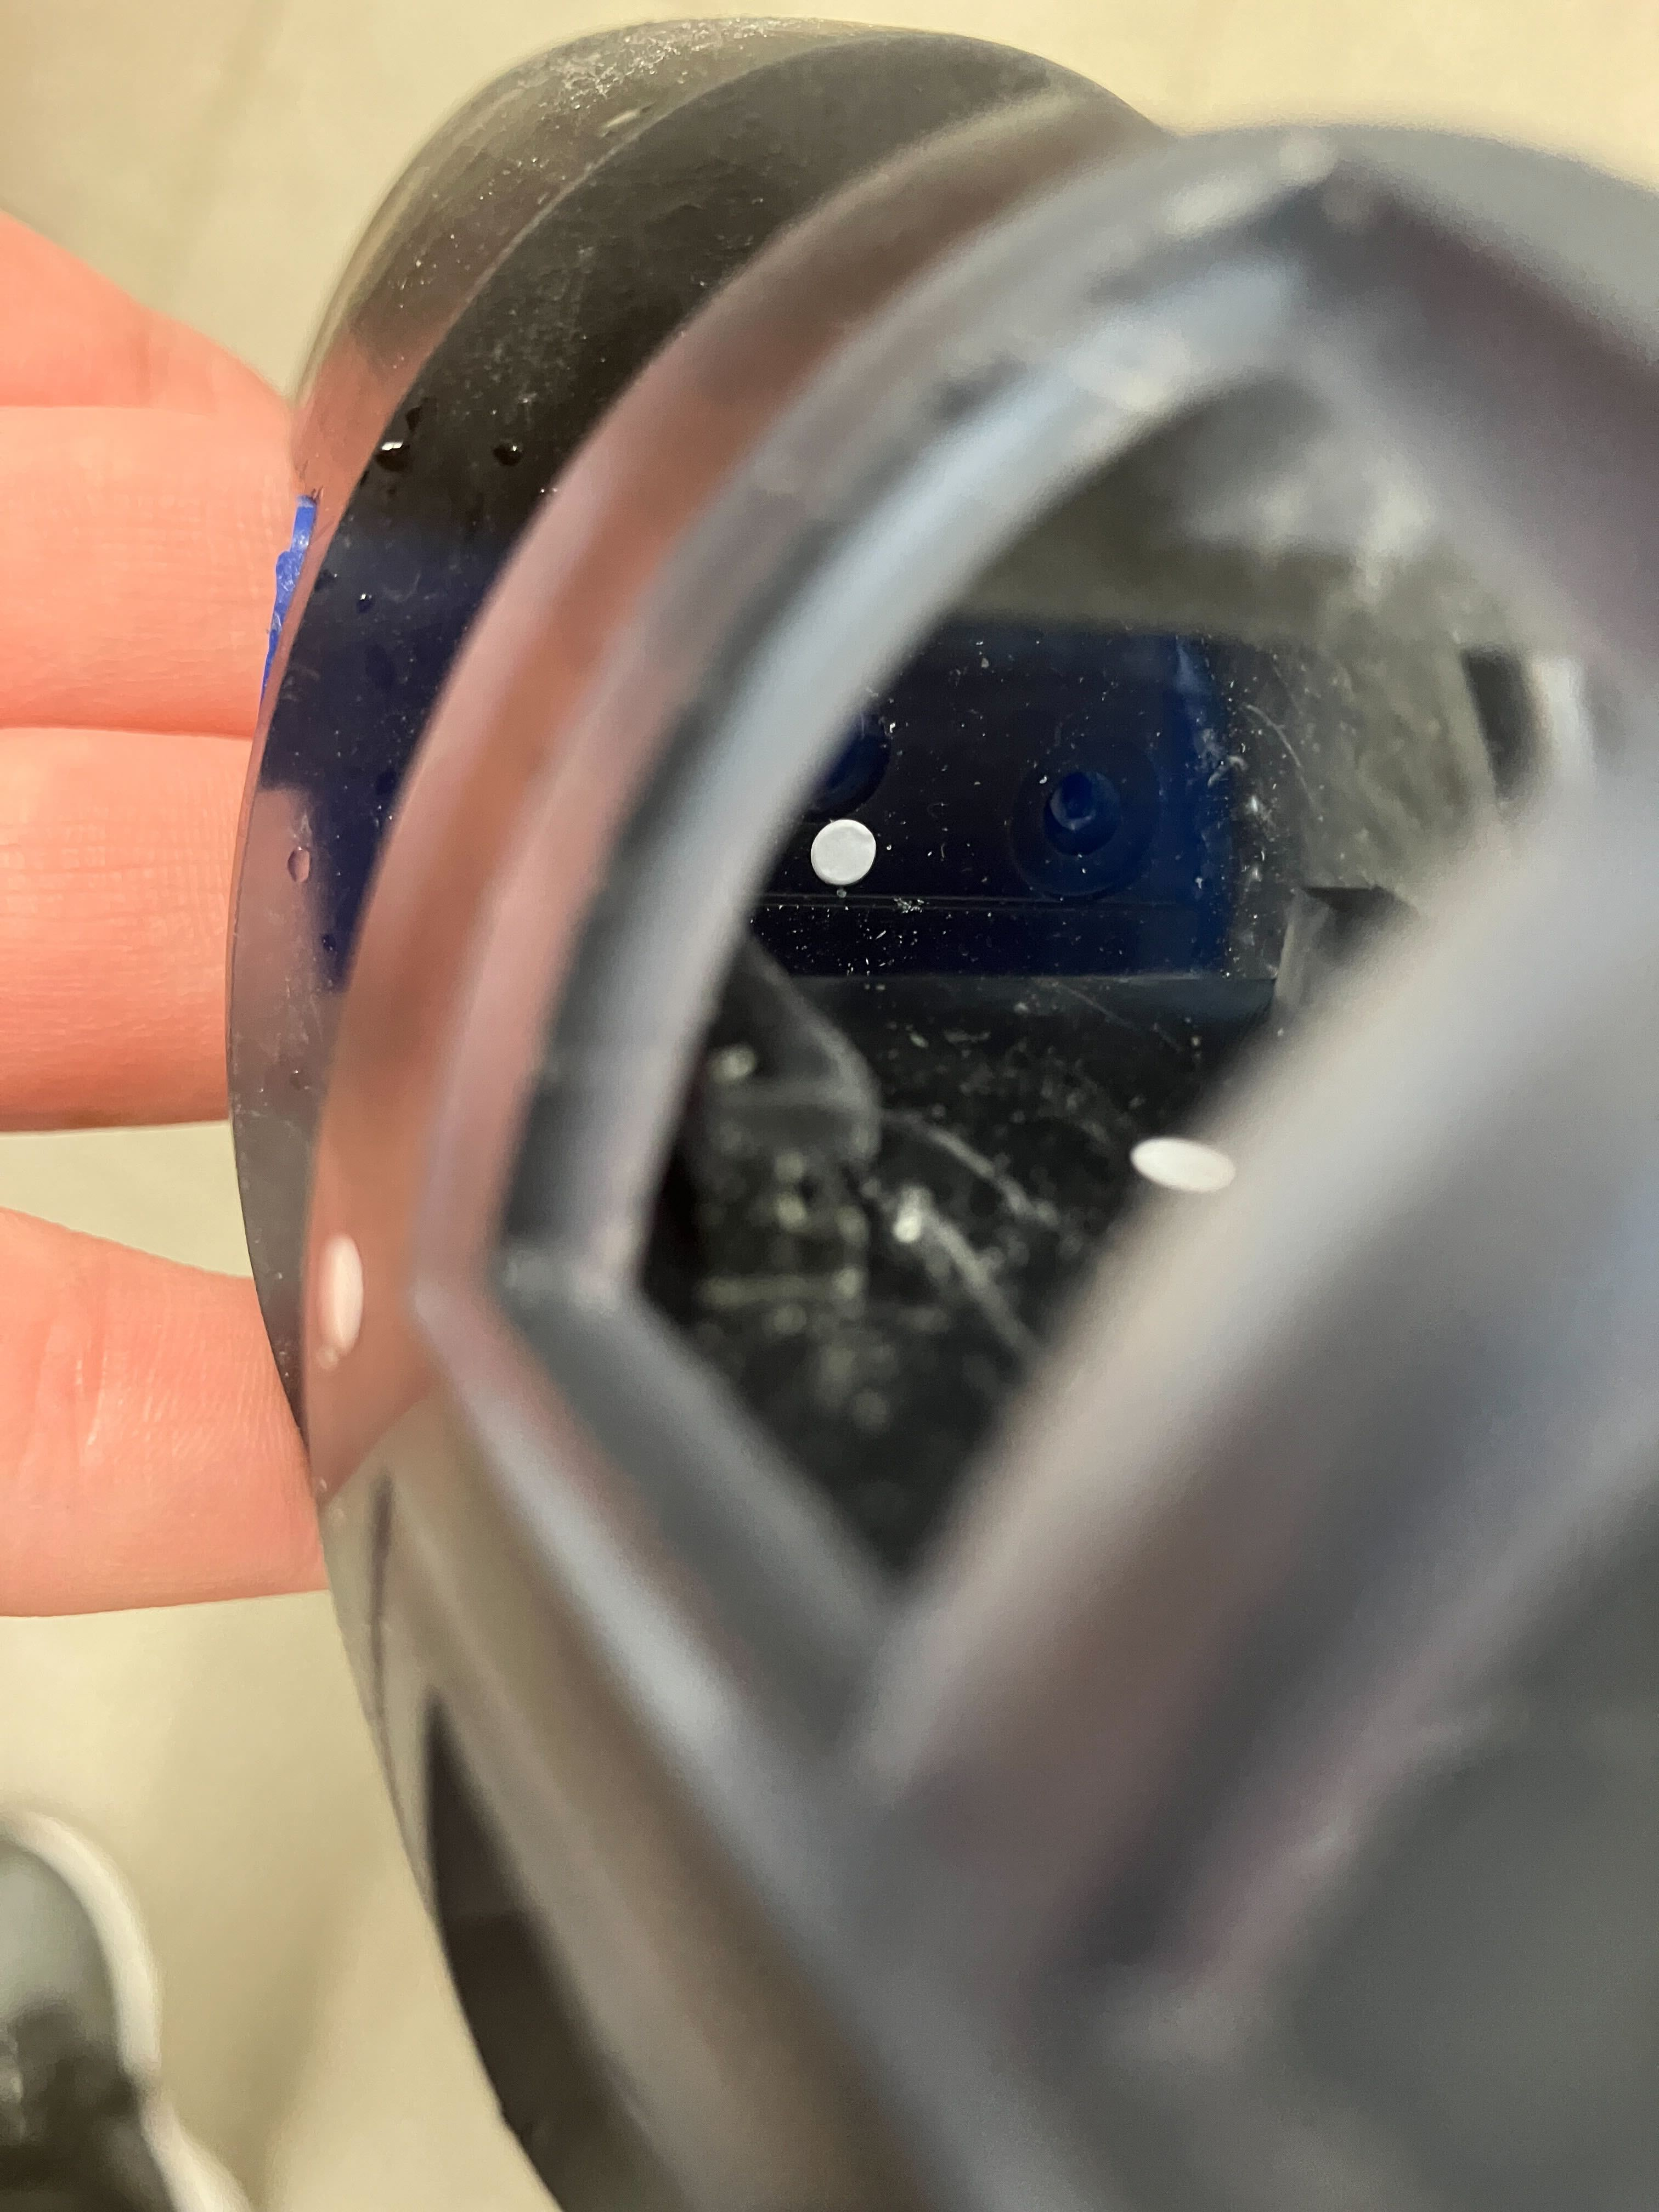
\includegraphics[width=0.7\linewidth]{chapters/picture/bousui_naka.jpg}
            \subcaption{頭部内側}
            \label{fig:toubu_uti}
        \end{minipage}
        \begin{minipage}[b]{0.25\linewidth}
            \centering
            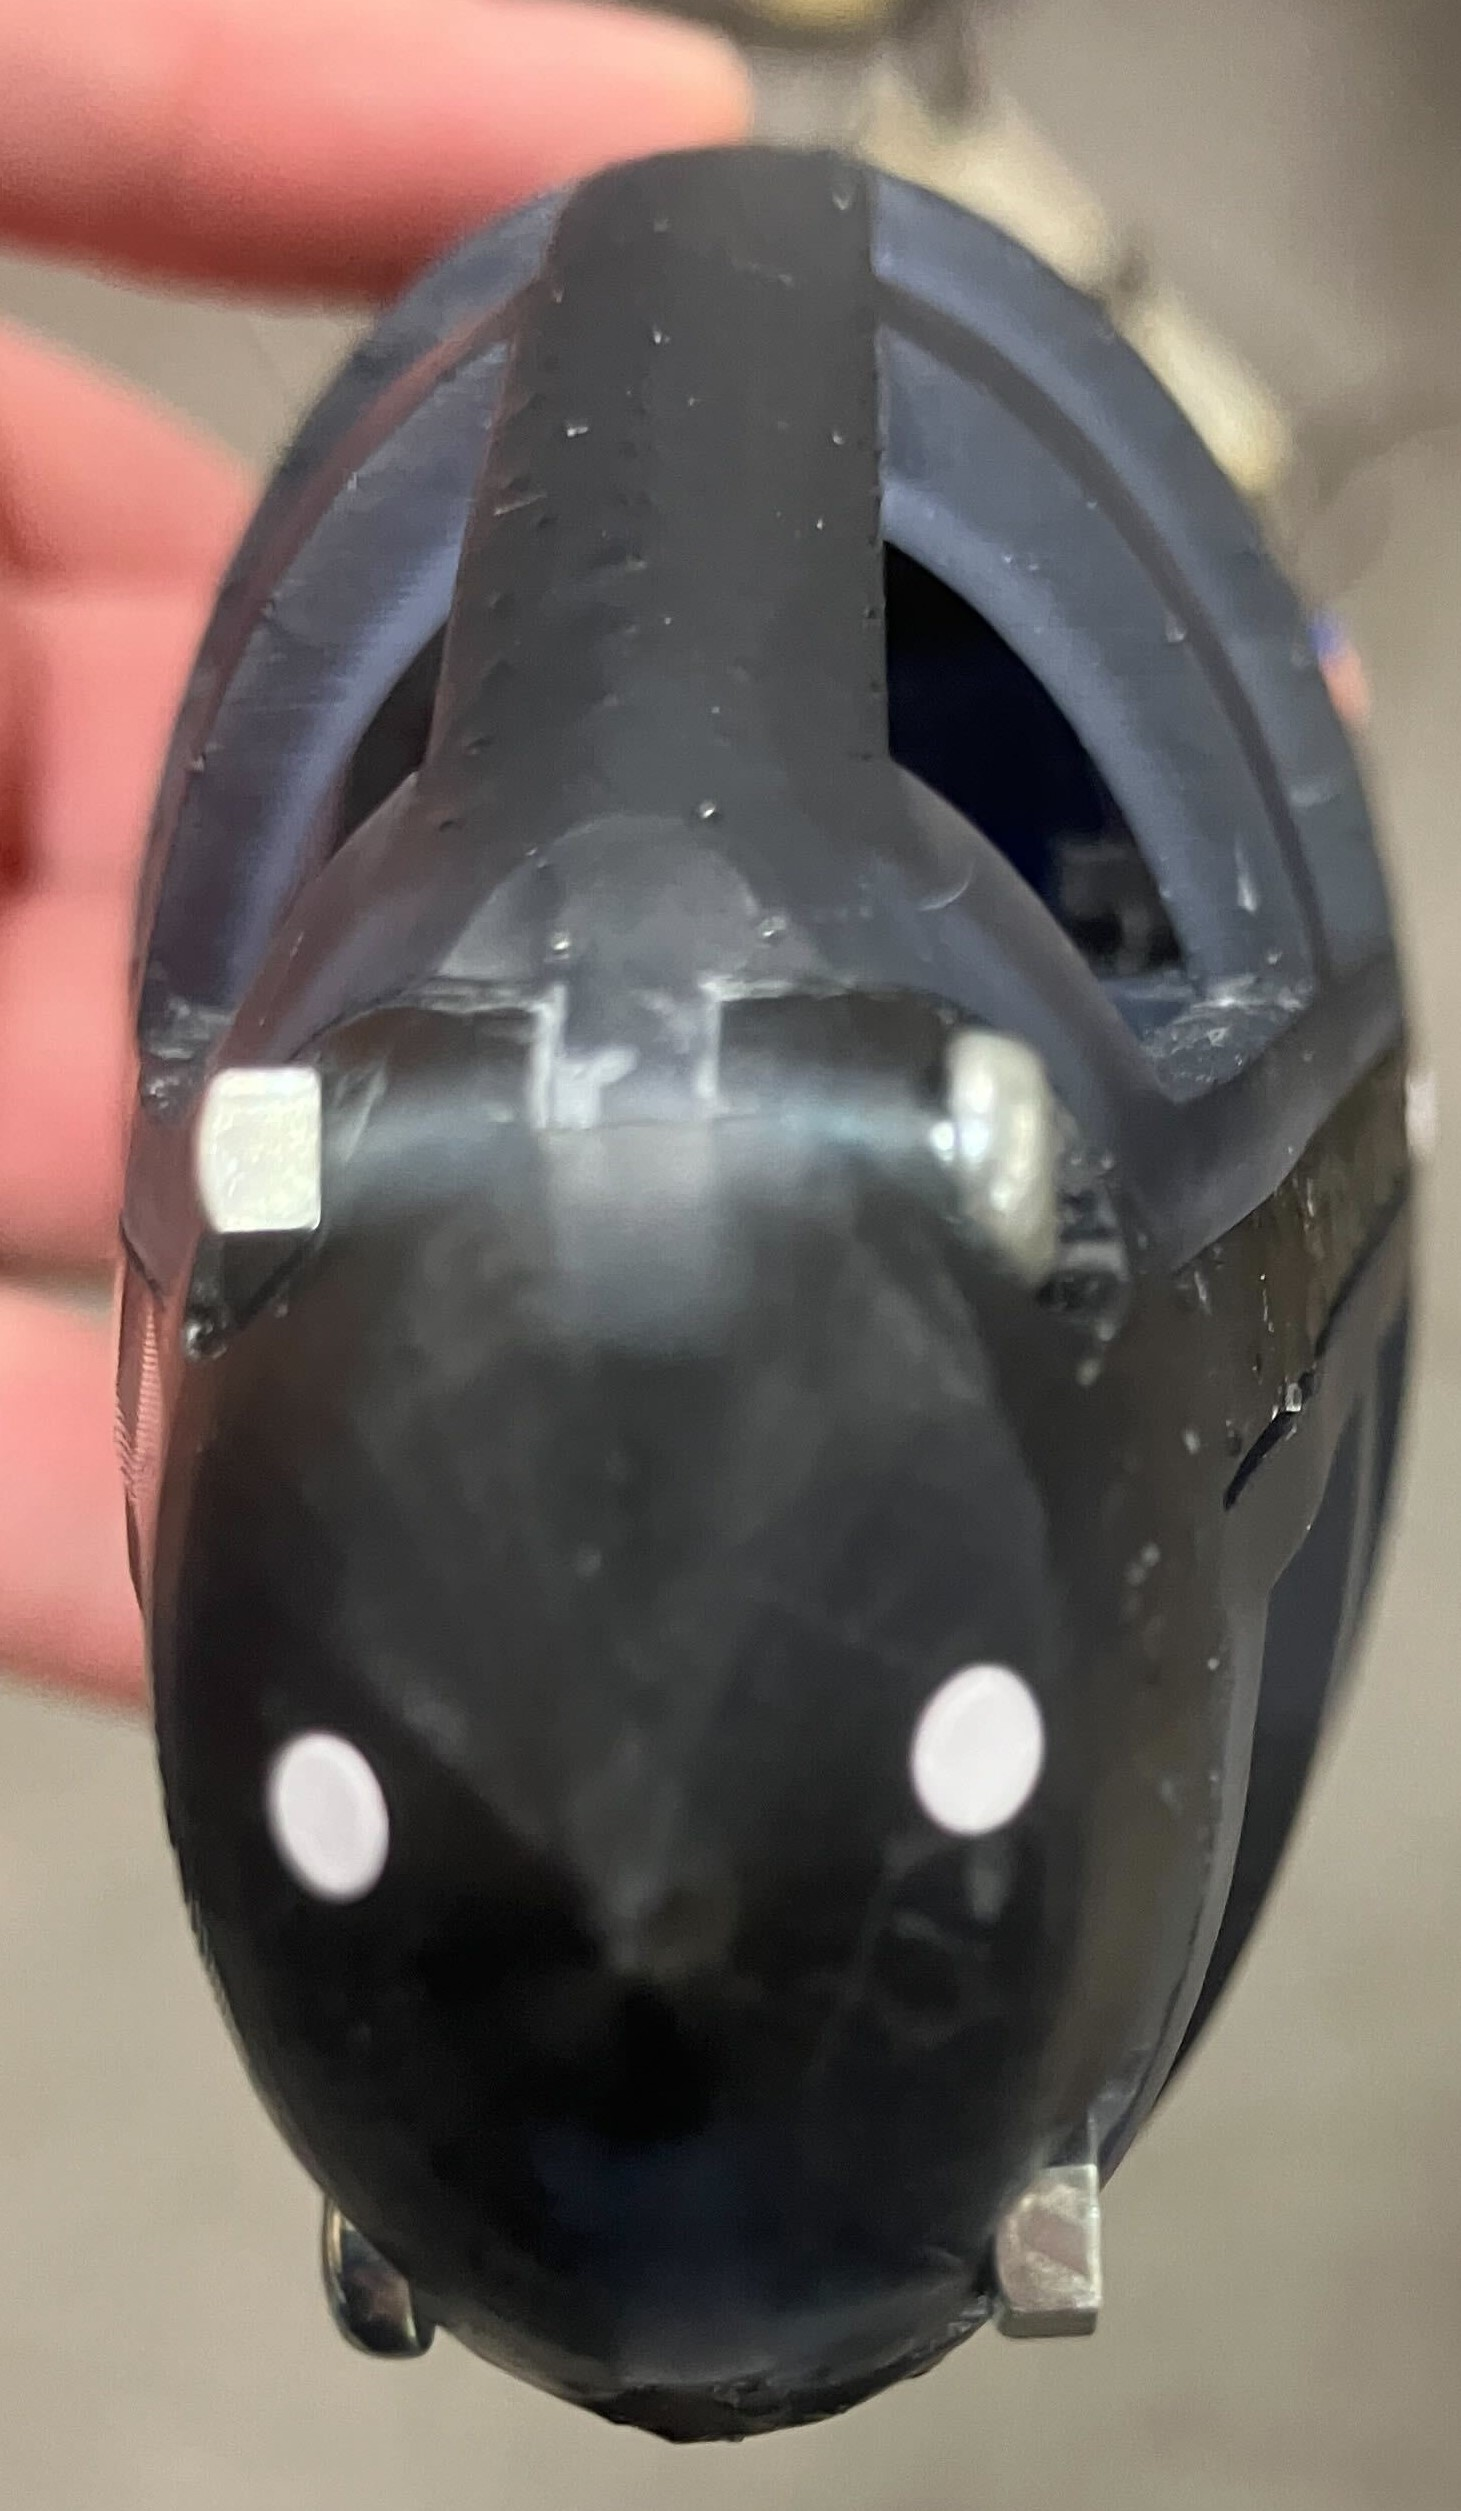
\includegraphics[width=0.6\linewidth]{chapters/picture/bousui_sentou.jpg}
            \subcaption{頭部先端}
            \label{fig:toubu_sentan}
        \end{minipage}
    \end{tabular}
    \caption{防水実験後のシールの様子}
    \label{fig:bousui_test}
\end{figure}
\begin{figure}[t]
    \centering
    \begin{minipage}[b]{0.3\linewidth}
        \centering
        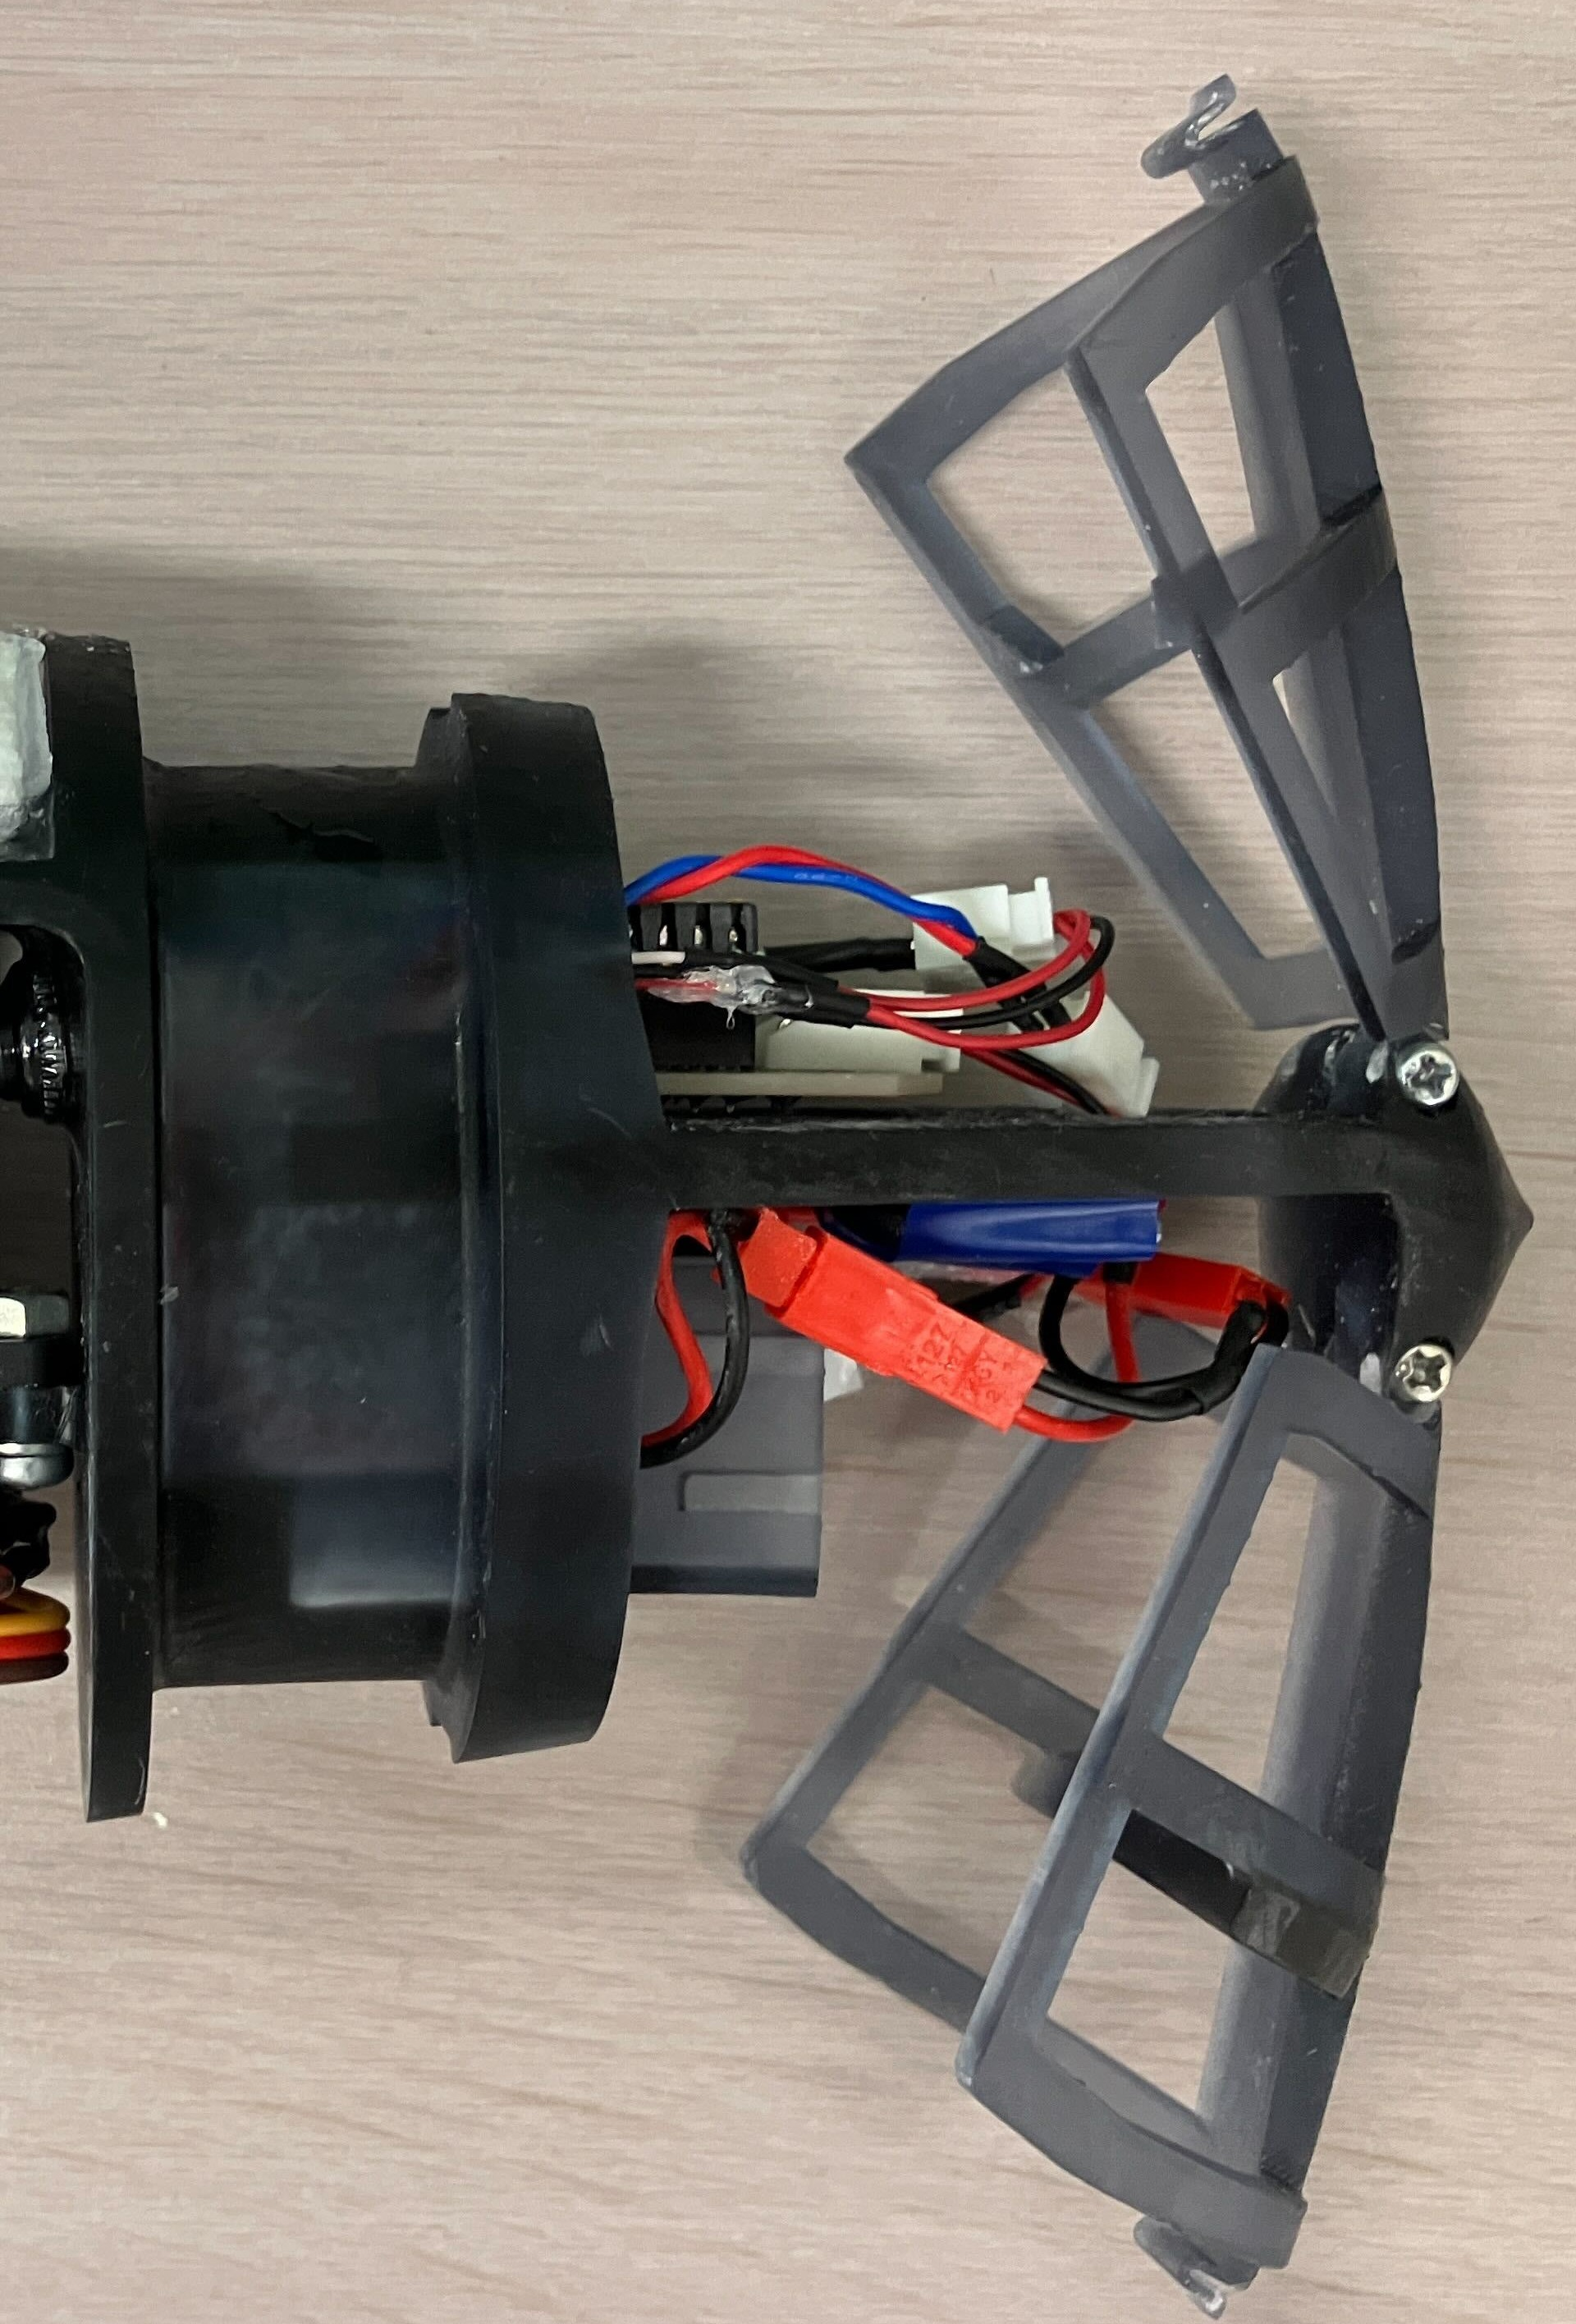
\includegraphics[width=0.4\linewidth]{chapters/picture/open_head.jpg}
        \caption{頭部全開時の様子}
        \label{fig:head_open}
    \end{minipage}
    \begin{minipage}[b]{0.44\linewidth}
        \centering
        \setPicture{rock.png}
        \caption{ワンタッチロックの仕組み}
        \label{fig:rock}
    \end{minipage}
\end{figure}
\begin{figure}[t]
    \centering
    \begin{minipage}[b]{0.35\linewidth}
        \centering
        \setPicture{toubu_kiban.png}
        \caption{基板固定方法}
        \label{fig:toubu_kiban}
    \end{minipage}
    \hspace{0.05\linewidth}
    \begin{minipage}[b]{0.35\linewidth}
        \centering
        \setPicture{toubu_battery.png}
        \caption{バッテリー固定方法}
        \label{fig:toubu_battery}
    \end{minipage}
\end{figure}

\subsection{胴体部}
胴体部は細かく分けて駆動部,弾性体部,尾びれ部で構成されている.
駆動部は頭部と一体化しており,試作機と同じサーボモータを配置し,プーリー(PLA樹脂)を取り付けている.昨年度卒業研究では頭部にサーボモータを配置していたが,今回は先行研究\cite{juu}で示さ
れた胴体後半部のみ体をしならせ遊泳するアジ型遊泳の特徴に従い,胴体後半部のみを屈曲できるような位置にサーボモータを配置した.
また,サーボモータの信号線を制御回路側につなげるために防水キャプコン(オーム電機,OA-WS04M-20/25)を配置し,さらに電源スイッチも配置している(図\ref{fig:kudou}).また,駆動部には
図\ref{fig:cover}のようなカバーをかぶせ魚らしい形状になるようにしている.

弾性体部は弾性体(ポリプロピレン板,厚さ0.75 mm)と骨格リンク(PLA樹脂),ワイヤ(ポリエステル製,0.40 mm)で構成している.骨格リンクは厚みを6mmで作製し,14 mm間隔を空
けながら配置した.リンクには図のようにワイヤを通すために2 mmの穴を4 カ所開けており,さらに胴体内部を浸水させるために大きめの穴を6 個開けている(図\ref{fig:link2}).また,リンクと弾性体は
ネジを用いて二点止めし,外皮の動きによってリンクがずれないように工夫した(図\ref{fig:real_link}).

尾びれ部は図\ref{fig:obire}のように尾びれ本体(ポリスチレン製薄板,厚さ0.3 mm)と骨格リンクの一部で構成している.尾びれに関しては先行研究\cite{ni}より推進性能が高いと示された材料と厚みを使用して
おり,形状に関してはアジの3Dスキャンデータからサイズを決定した.
\begin{figure}[hb]
    \centering
    \begin{minipage}[b]{0.32\linewidth}
        \centering
        \setPicture{kudou.png}
        \caption{駆動部}
        \label{fig:kudou}
    \end{minipage}
    \hspace{0.1\linewidth}
    \begin{minipage}[b]{0.3\linewidth}
        \centering
        \setPicture{cover.jpg}
        \caption{駆動部カバー}
        \label{fig:cover}
    \end{minipage}
\end{figure}
\begin{figure}[hb]
    \centering
    \begin{minipage}[b]{0.30\linewidth}
        \centering
        \setPicture{link2.png}
        \caption{骨格リンク}
        \label{fig:link2}
    \end{minipage}
    \hspace{0.1\linewidth}
    \begin{minipage}[b]{0.33\linewidth}
        \centering
        \setPicture{link_danseita.jpg}
        \caption{弾性体部}
        \label{fig:real_link}
    \end{minipage}
\end{figure}
\begin{figure}[t]
    \centering
    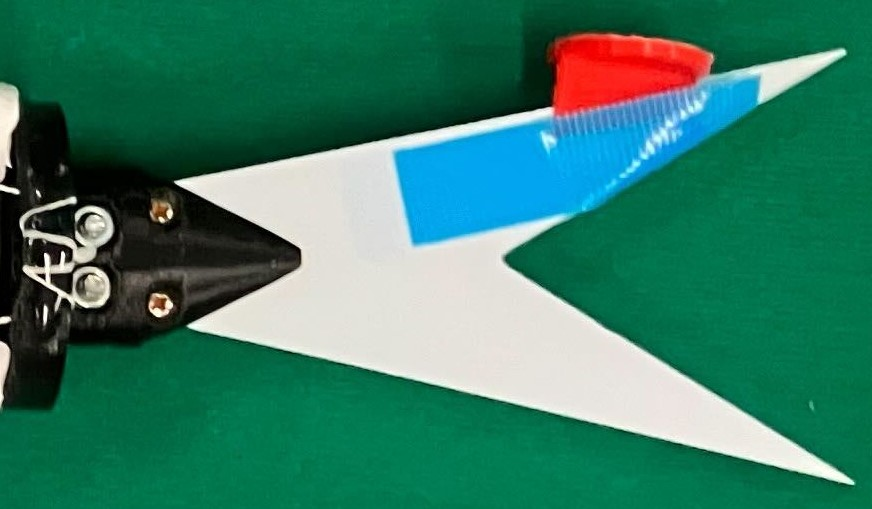
\includegraphics[width=0.5\linewidth]{chapters/picture/obire.jpg}
    \caption{尾びれ部}
    \label{fig:obire}
\end{figure}
骨格リンクは尾びれを固定するための固定部を設け,尾びれが折れないようにTPU樹脂で作製し,根元を三角形状にすることで折り目がつ
かないようにした.また,尾びれにはトラッキング用のマーカー(PLA樹脂)を取り付けた.

\subsection{柔軟外皮}
柔軟外皮は頭部と胴体部用に二つ作製した.今回は先行研究\cite{kyu}を参考に柔軟外皮を作製するため鋳造のように型にシリコン(Smooth-On社,ECOFLEX30)を流し入れることによって柔軟外皮の作製を行った.図\ref{fig:katanaka}に作製・使用した型
と中子をそれぞれ示す.ここで中子とは鋳造において中空部を作るために使われているもので, 型の間にはめ込んで使用する.この製作方法において柔軟外皮の外寸サイズを決定するのは型に作る
くぼみ,内寸サイズを決定するのは中子となる.したがってここから型のくぼみのサイズを柔軟外皮の外寸,中子のサイズを柔軟外皮の内寸と呼ぶ.

まず頭部用の柔軟外皮について,柔軟外皮の内寸は柔軟外皮と頭部が密着するようにアジの3Dモデルの頭部のサイズをそのまま使用した.外寸については体高方向に2 mm,体幅方向に3 mmの厚みになるよう
にアジのモデルデータの頭部をx軸方向に1.15 倍,y軸方向に1.09 倍,z軸方向に1.07 倍したサイズを使用した.

次に胴体部の柔軟外皮ついて述べる.リンクの動きに柔軟外皮を追従させるために柔軟外皮内部に骨格リンクをはめ込めるような溝を作製し,しわができないように柔軟外皮の内寸をロボットの胴体サイズの90 %
のサイズで作製した.サイズを小さめに作製することにより常に外皮にテンションがかかり,しわが寄らないようになった.溝の間隔もロボット胴体サイズの90 %になるようにリンク間距離14 mm
の90 %の長さにあたる12.6 mm間隔で作製した.溝の深さは骨格リンクに通すワイヤに干渉しないかつ溝から外れないように5 mmで設計した.
図\ref{fig:gaihi}に作製した柔軟外皮を示す.

胴体部の柔軟外皮はリンクを溝にはめ込むことである程度固定される.また柔軟外皮の頭部側の端を防水リングを締め付ける溝の部分にひっかける事によってさらに固定をしている(図\ref{fig:gaihi_kotei}の
赤丸の部分がひっかけている箇所).
\begin{figure}[t]
    \centering
    \begin{tabular}{cc}
        \begin{minipage}[b]{0.4\linewidth}
            \centering
            \setPicture{atata.jpg}
            \subcaption{頭部の柔軟外皮用の型と中子}
            \label{fig:atata} 
        \end{minipage}
        \hspace{0.05\linewidth}
        \begin{minipage}[b]{0.4\linewidth}
            \centering
            \setPicture{katata.jpg}
            \subcaption{胴体部の柔軟外皮用の型と中子}
            \label{fig:katata} 
        \end{minipage}
    \end{tabular}
    \caption{作製した型と中子}
    \label{fig:katanaka}
\end{figure}
\begin{figure}[ht]
    \centering
    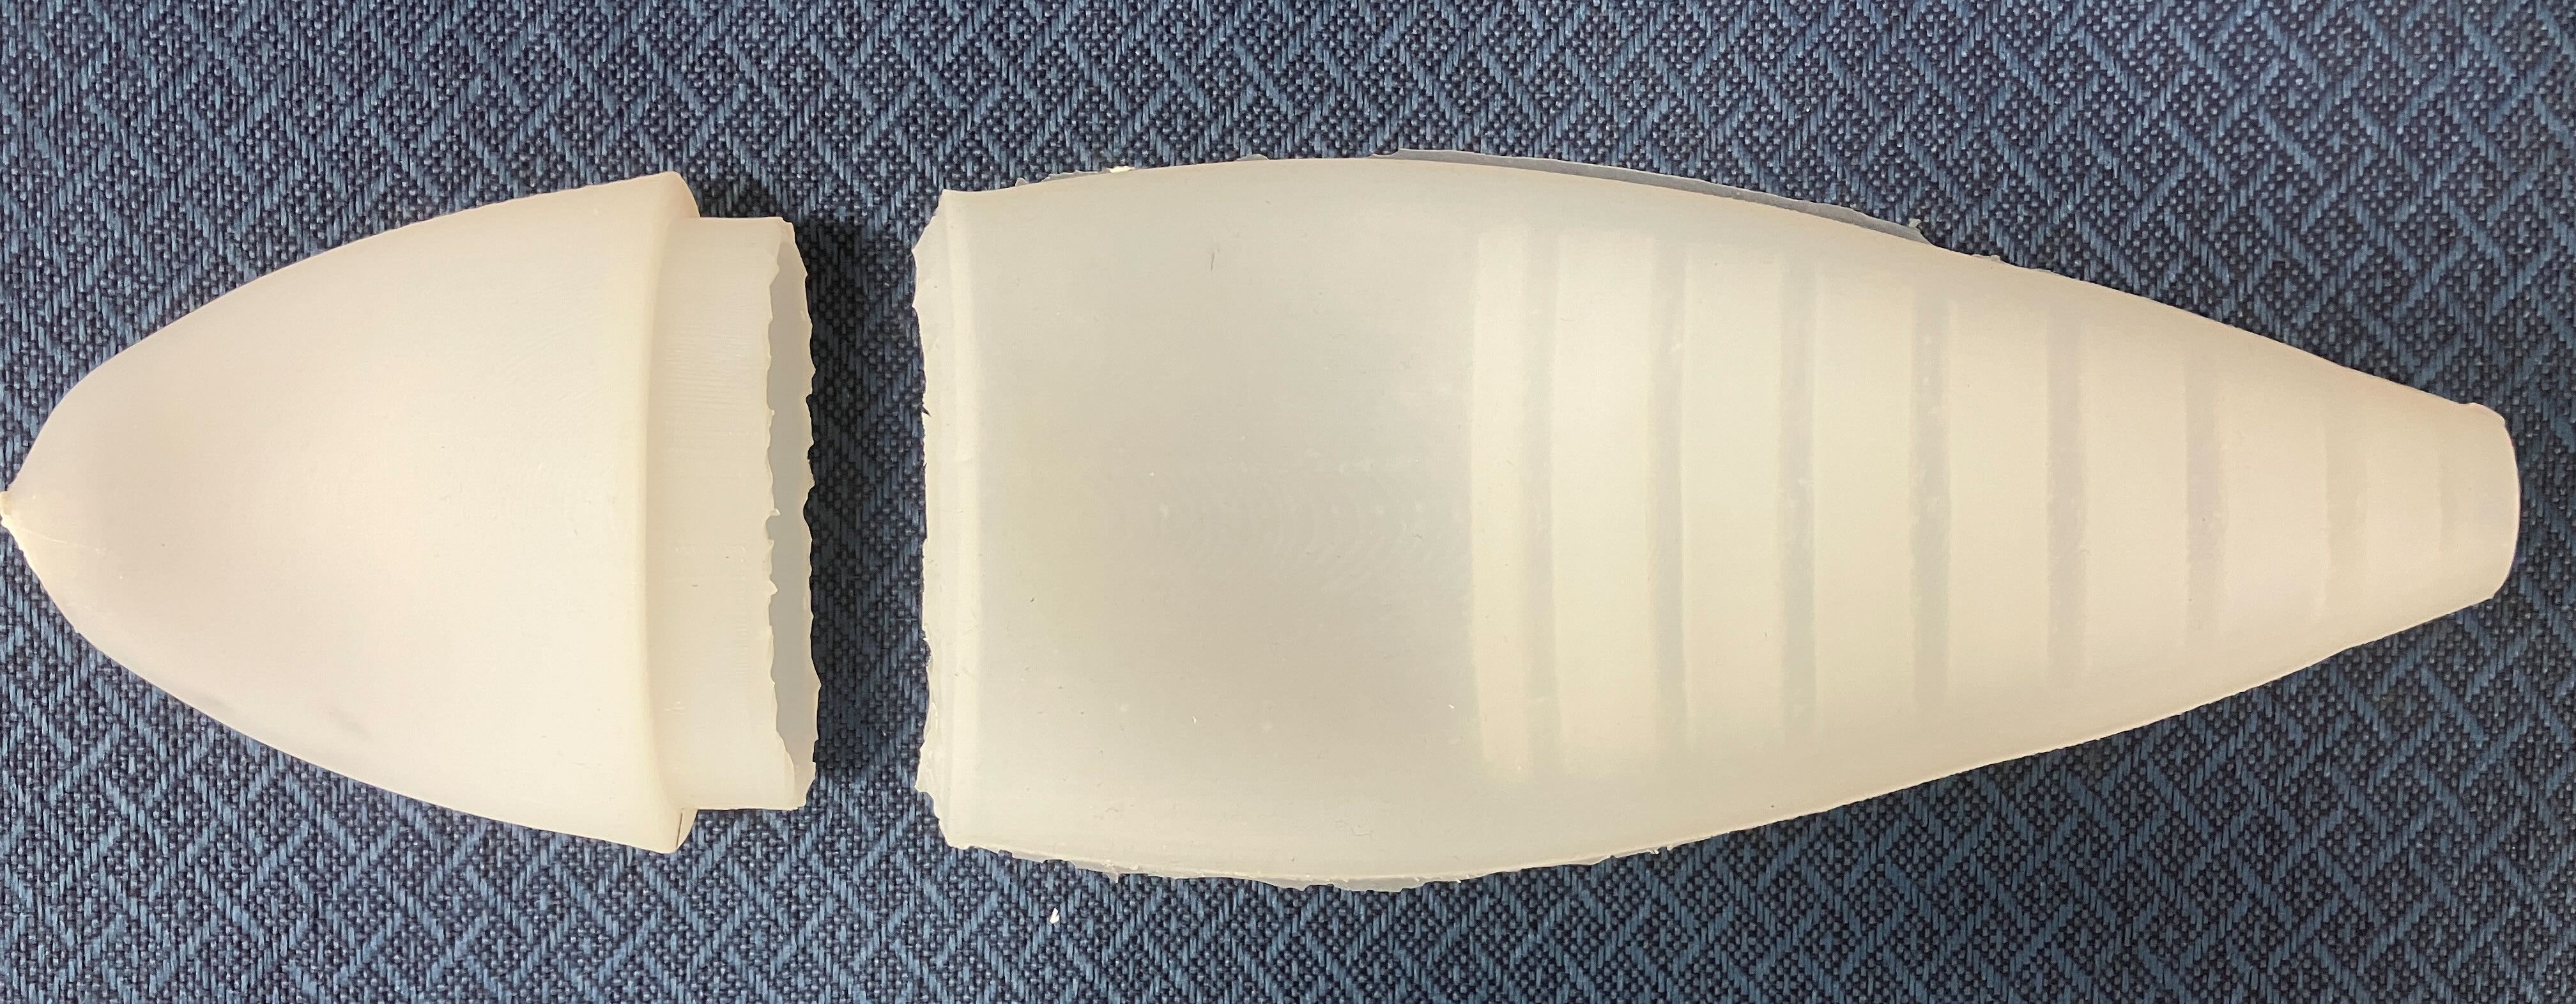
\includegraphics[width=0.8\linewidth]{chapters/picture/gaihi.jpg}
    \caption{作製した外皮}
    \label{fig:gaihi}
\end{figure}
\begin{figure}[t]
    \centering
    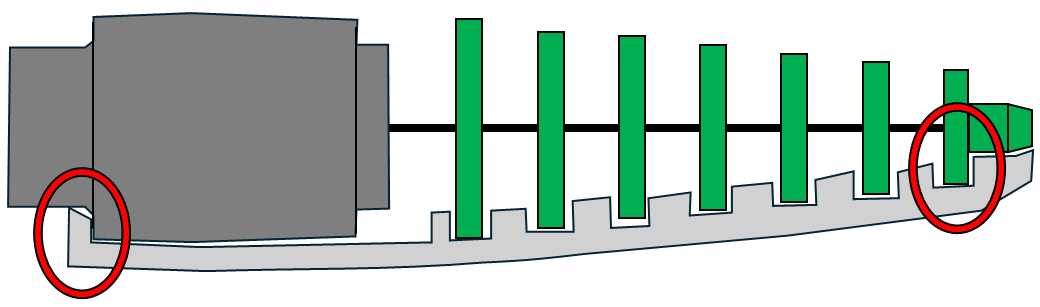
\includegraphics[width=0.7\linewidth]{chapters/picture/gaihi_kotei.png}
    \caption{胴体部の柔軟外皮の固定}
    \label{fig:gaihi_kotei}
\end{figure}
\newpage
\section{遊泳実験}
外皮の有無による遊泳性能への影響を検証するために,胴体外皮未装着時と胴体外皮装着時それぞれで直進遊泳実験を行った.図\ref{fig:doutainasi}に胴体外皮未装着時の状態を示す.

\subsection{実験条件}
サーボモータには昨年度卒業研究と同様にステップ上の入力を与えた(図\ref{fig:servo_seigyo}).$T$ [ms]は入力の周期,$\theta$ [deg]はプーリの回転角(糸の巻き取り量)を表してい
る.ここでこの実験で使用する尾びれ周波数と尾びれ振幅という二つのパラメータをついて述べる.まず尾びれ周波数は尾びれを振る速さを決定するパラメータであり,$f = 1/T$ [Hz]で算出する.
尾びれ振幅は体をどのくらい屈曲させるかのパラメータであり,トラッキングソフト「kinovea」を用いて尾びれの振れ角を算出し,それを尾びれ振幅とした(図\ref{fig:obire_amp}). 

直進遊泳実験は尾びれ振幅を一定にし,尾びれ周波数を変更した時の速度を測定した.尾びれ振幅はプーリの回転角を$30\:^\circ$,$45\:^\circ$,$60\:^\circ$としたときのそれぞれのトラッ
キング角度$81\:^\circ$,$114\:^\circ$,$168\:^\circ$で一定にし,尾びれ周波数は0.5~1.75 Hzまで0.25 Hzずつ変化させ,合計54 個のパラメータについて実験を行った.
各パラメータにつき3回実験を行い,得られた遊泳速度のデータから平均,分散,標準偏差を算出した.
\begin{figure}[htbp]
    \centering
    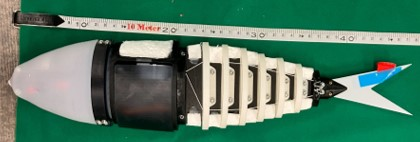
\includegraphics[width=0.8\linewidth]{chapters/picture/without_skin.jpg}
    \caption{胴体外皮未装着の状態}
    \label{fig:doutainasi}
\end{figure}
\begin{figure}[htbp]
    \centering
     \begin{minipage}[b]{0.5\linewidth}
        \centering
        \setPicture{servo.png}
        \caption{サーボへの制御入力}
        \label{fig:servo_seigyo}
     \end{minipage}
     \hspace{0.05\linewidth}
     \begin{minipage}[b]{0.4\linewidth}
        \centering
        \setPicture{obire_amp.png}
        \caption{尾びれ振幅について}
        \label{fig:obire_amp}
     \end{minipage}
\end{figure}
次に遊泳速度の算出方法について述べる.まずは天井に取り付けたカメラを用いて撮影した動画から尾びれに取り付けたマーカーをkinoveaでトラッキングする.そして得られた尾びれ軌跡のトラッキングデータ
を二次近似し,積分して遊泳距離を算出し,遊泳時間で除算して遊泳速度を算出する.直進遊泳開始時に過渡状態となることを踏まえ,トラッキング範囲を遊泳を開始してから500~1500 mmの範囲に設定した.

\subsection{実験結果}
図に振幅,周波数の時の遊泳実験の様子を,図に実験結果を示す.図のエラーバーは算出した標準偏差を示している.遊泳実験では,すべてのパラメータで直進させたかったが,何回か進行方向が右に傾いたり左
に傾いたりしてしまう時があった.図から,まず外皮あり・なし両方に共通して周波数が高くなるほど



\newpage
\subsection{考察}
まず,外皮アリ・ナシで尾びれの振りに差が出てしまったことについて考察する.原因としては外皮に作った溝が胴体の屈曲を阻害し,本来胴体が屈曲するはずだった
位置まで動くことができなかったと考えられる(図\ref{fig:sogai}).実際に外皮を装着した状態で空中で振幅を測定してみる.測定した結果,プーリの回転角が$30\:^\circ$,
$45\:^\circ$,$60\:^\circ$のとき,尾ビレ振幅はそれぞれ$81\:^\circ$,$88\:^\circ$,$128\:^\circ$となった.本来の尾びれ振幅$81\:^\circ$,
$114\:^\circ$,$168\:^\circ$と比較すると約$40\:^\circ$差があるのがわかる(表\ref{tb:amp}).しかしここで外皮ナシと外皮アリで角度が比較的近い$81\:^\circ$と
$88\:^\circ$で比較しても実験結果と同じように外皮装着時のほうが速度が速くなっているので実験結果に影響を与えてしまうものではないと考える.
さらに言えば外皮アリの時の尾びれ振幅を実際の角度に近づけて実験を行えば,今回の結果よりもより優れた遊泳性能を示す実験結果を得ることができるといえる.

次に遊泳時に進行方向が傾いたことについて考察する.昨年度卒業研究ではワイヤーが左右に偏ることによって進行方向が傾いていたため,今回の実験では,ワイヤーの張力が左右に
偏ることを防ぐために,サーボモータの基準角度を変更してワイヤーの張力が偏らないようにプログラムを組んでいた.しかし,基準角をプログラムで調整しても進行方向が少し傾いて
しまったり,遊泳実験をしている最中に今まで直進していた設定の時に進行方向が曲がってしまうことがあった.
原因として考えられることは2つある.1つ目は外皮を装着することによって胴体を屈曲させるためのトルクが増大し,
\begin{table}[htbp]
    \centering
    \caption{サーボ巻き取り角と尾びれ振幅の関係}
    \label{tb:amp}
    \begin{tabular}{|c||c|c|}\hline
        サーボ巻き取り角[deg]&実験で使用した振幅[deg]&外皮装着時の振幅[deg]\\ \hline
        30&81&n\\ \hline
        45&114&88\\ \hline
        60&168&128\\ \hline
    \end{tabular}
\end{table}
\begin{figure}[hb]
    \centering
    \begin{tabular}{cc}
        \begin{minipage}[b]{0.4\linewidth}
            \centering
            \setPicture{gaihi_jama_nasi.png}
            \subcaption{外皮未装着時の胴体屈曲状態}
            \label{fig:jama_nasi}
        \end{minipage}
        \hspace{0.1\linewidth}
        \begin{minipage}[b]{0.4\linewidth}
            \centering
            \setPicture{gaihi_jama.png}
            \subcaption{外皮装着時の胴体屈曲状態}
            \label{fig:jama}
        \end{minipage}
    \end{tabular}
    \caption{外皮による屈曲の阻害}
    \label{fig:sogai}
\end{figure}
それに伴って糸が伸びた,またはたるんでしまったということが考えられる.
2つ目はスタート時の姿勢が若干左右どちらかに傾いてしまったことにより,結果として左右に進行方向が傾いているように見えたと考えられる.
改善策として,糸の張力を一定にできる治具をロボットに取り付ける,もしくは使用するワイヤを現在使用しているワイヤよりも強度が高いものにするといったことがあげられる.

次に外皮ナシの状態の時に振幅の変化によってそこまで速度にそこまで大きな変化が無かったことについて考察する.外皮無しで振幅$168\:^\circ$,周波数1.75 Hz時の遊泳時
の様子を見てみると(図\ref{fig:teikou})推進時に体が大きく屈曲してしまい,進行方向からの抵抗力を頭部と胴体部の一部で受けてしまっていることが分かる.これによっ
て本来その振幅で得られるはずだった推進力が低減し,遊泳速度が振幅によって変化しなかったと考えられる.
\begin{figure}[t]
    \centering
    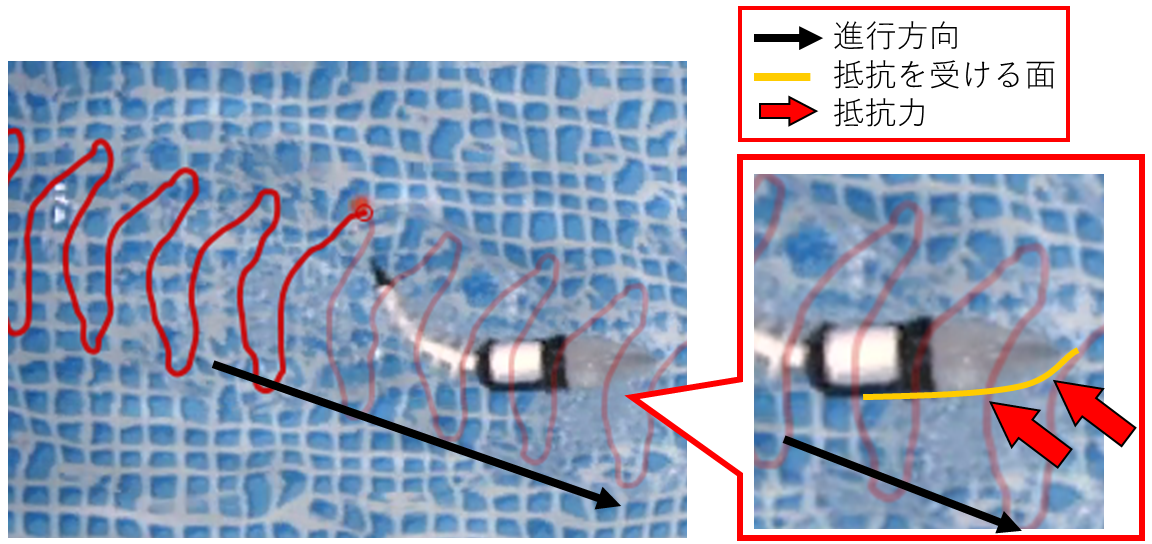
\includegraphics[width=0.9\linewidth]{chapters/picture/teikou.png}
    \caption{外皮未装着時に受ける抵抗}
    \label{fig:teikou}
\end{figure}
\begin{figure}[t]
    \centering
    \begin{tabular}{cc}
        \begin{minipage}[b]{0.45\linewidth}
            \centering
            \setPicture{compare_withoutskin.eps}
            \subcaption{外皮未装着時}
            \label{fig:without_matome}
        \end{minipage}
        \begin{minipage}[b]{0.45\linewidth}
            \centering
            \setPicture{compare_withskin.eps}
            \subcaption{外皮装着時}
            \label{fig:withskin_matome}
        \end{minipage}
    \end{tabular}
    \caption{外皮未装着時・装着時の結果をまとめたグラフ}
    \label{fig:matome}
\end{figure}
次に高周波数域において外皮が遊泳性能に与える影響について考察する.図\ref{fig:matome}に外皮有り・無しそれぞれの結果を一つのグラフにまとめたものを示す.グラフから低周波数域において
は外皮有り・無し両方において振幅による速度の変化はそれほど大きくは無かった.しかし,高周波数域を見てみると,外皮未装着時では振幅によってそこまで遊泳速度に差がない
のに対し,外皮装着時は振幅が大きくなるほど遊泳速度に差が出ていることが分かる.このことから高周波数域において柔軟外皮は遊泳性能に大きな影響を与えると考えられる.

\begin{figure}[t]
    \centering
    \setPicture{body.pdf}
    \caption{外皮の有無によるボディの違い}
    \label{fig:body}
\end{figure}

最後に外皮を装着することによってなぜ遊泳速度が向上したのかについて考察する.要因として考えられるのは外皮装着時と未装着時でボディが異なっていることである.外皮未装着時のボディは半流
線型のボディになっているのに対し,外皮装着時は流線型のボディになっている(図\ref{fig:body}).ここで流線型のボディはほかの形状に比べて物体の正面と背面の圧力差によって生じる圧力抵抗を低減することができ
る.したがって,ロボットのボディを流線型にすることによって水中で受ける抵抗力が減り,その分推進力が増大したと考えられる.
このことから,魚型ロボットに流線型のボディを備えることは遊泳性能の向上につながるといえる.

\subsection{今後の展望}
本研究では魚ロボットを用いて直進湯上実験を行い,結果としてリンクの動きに追従できる柔軟外皮の開発に成功し,外皮によって遊泳速度が向上することも確かめられた.しかし,外皮によって胴体の屈曲が阻害され,
目的の振幅を得られないという問題があった.外皮内部に作る溝の幅ををあえてリンクより広めの幅で作製するか,サーボモータをより高トルクなものに変更することで解決できると考えられる.また,本実験では防水
処理を施されていたサーボモータが2回水没してしまったので,防水規格がIP68のモータに変更した方がよいと考える.また,本研究の実験結果から外皮装着時は周波数が高く,振幅が大きいほど遊泳速度が向上すると
いうことがわかったが,さらに速い速度で遊泳させるために1.75Hz以上の周波数で遊泳を行うと,サーボモータが指令角度に到達する前に次の動作に移り,結果として振幅が小さくなってしまう可能性がある.そこで
今後はより多くの周波数で実験が可能になるようにサーボモータよりもより細かな制御が可能なブラシレスDCモータを使用し,遊泳速度の向上を図りたい.
また,本研究では直進性能しか検証できていないため,急旋回実験を行って旋回速度や旋回角度などの旋回性能を検証したい.
そして最終的には柔軟外皮の表面にウロコを配置し,対衝撃性能や遊泳性能への影響を検証し,魚らしい見た目を持った高機動性を有する魚ロボットの開発を目指す.
% 必要に応じて章を増やす,またファイル名もsec2, sec3である必要はない
% このmain.texが置いてあるディレクトリ内にある「chapters」フォルダ以下に
% 自分がわかりやすい名前のtexファイルを作成し,\include{chapters/*****}で
% 呼び出せば良い
\newpage
\section{結言}
本研究では,魚らしいしなやかな動きを可能にするワイヤ駆動式の魚ロボットをベースにリンクに外皮を追従させ,尾びれのみならず
胴体部まで振って泳ぐことが可能なロボットの開発を行った.そして実験結果から

      % 結言
\newpage
\section{謝辞} % 謝辞
% できればbibtexを使ってください

\newpage
\section{参考文献}
\begin{thebibliography}{9}
    \bibitem{ichi}
    平田宏一, 春海一佳, 瀧本忠教, 田村兼吉, 牧野雅彦, 児玉良明, 冨田宏. 魚ロボットに関する基礎的研究. 海上技術安全研究所報告, Vol. 2, No. 3, pp. 281-307, 2003.
 
    \bibitem{ni}
    高田洋吾, 中西志允, 荒木良介, 脇坂知行. Piv 測定と3 次元数値解析による小型魚ロボット周りの水の流動状態と推進能力の検討(機械力学, 計測, 自動制御). 日本機械学会論文集C 編, Vol. 76, No. 763, pp. 665–672, 2010.

    \bibitem{san}
    高田洋吾, 中村毅志, 小山圭介, 田尻智紀. 色情報に基づく小型魚ロボットfocus の目標物追従制御. 日本機械学会論文集C 編, Vol. 78, No. 792, pp. 2924–2934, 2012.

    \bibitem{yon}
    中西大輔, 山根拓真, 末岡裕一郎, モータ・ワイヤ駆動併用型飛び移り座屈機構を用いた魚型ロボットの開発, ロボティクス・メカトロニクス講演会2020, 1P1-C04, 2020

    \bibitem{go}
    末岡裕一郎, 花原健太郎, 中西大輔, 大須賀公一. ワイヤ駆動の飛び移り座屈機構を搭載した魚型ロボットの大振幅遊泳. ロボティクス・メカトロニクス講演会講演概要集2020, 1P1–C05. 一般社団法人日本機械学会, 2020.

    \bibitem{roku}
    板垣達也, 中西大輔. しなやかな胴体を有する飛び移り座屈駆動式魚型ロボットの開発.ロボティクス・メカトロニクス講演会講演概要集2021, 2P3–H10. 一般社団法人日本機械学会, 2021.

    \bibitem{nana}
    中西大輔, 吉岡祐亮, ワイヤ駆動と連続飛び移り座屈機構を併用した魚型ロボットの開発, 第23回 公益社団法人 計測自動制御学会システムインテグレーション部門講演会, 1P3-H05, 2022.

    \bibitem{hachi}
    中西 大輔,高橋 海成,飛び移り座屈駆動式魚型ロボットによる旋回遊泳の実現, 第24回計測自動制御学会システムインテグレーション部門講演会(SI2023), 2C4-05, 2023.

    \bibitem{kyu}
    中西大輔, 石原康平, 柔軟外皮を有する飛び移り座屈駆動式魚型ロボットの開発. ロボティクス・メカトロニクス講演会2024, 2P2-B10, 2024.

    \bibitem{juu}
    神部勉, 魚の運動と渦. nagare, 1976, 8.3: 2-10.

    \bibitem{juuiti}
    朝日電装株式会社, "シール技術", 要素技術, \url{https://www.ad-asahidenso.co.jp/technology/water-proof_dust-proof/sealing/}, (参照 2024-12-13)

\end{thebibliography}


    % 参考文献

\end{document}
